% !TeX spellcheck = en_US
% !TeX encoding = UTF-8

\documentclass[
	paper=A4,
	twoside=true,
	openright,
	parskip=full,
	chapterprefix=true,
	12pt,
	headings=normal,
	bibliography=totoc,
	listof=totoc,
	titlepage=on,
%	draft
	final
	]{scrreprt}

\usepackage{lieb}
\graphicspath{{images/}}

\title{Discovery Potential of a Model Independent Search for New Physics at the LHC}
\date{\today}
\author{Jonas Lieb}

\makeatletter
\let\theauthor\@author
\let\thetitle\@title
\let\thedate\@date
\makeatother

\hypersetup{
	pdftex,
	pdfauthor={\theauthor},
	pdftitle={\thetitle},
	pdflang={en-US},
	pdfcreator={},
	pdfproducer={},
}

\begin{document}

\cleardoublepage
\pagenumbering{roman}
\pagestyle{empty}

% mark ATLAS as accronym used before
\acused{ATLAS}

% !TeX spellcheck = de_DE
% !TeX encoding = UTF-8
% !TeX root = ../document.tex

\makeatletter
\begin{titlepage}
		\tgherosfont
		\centering
		
		\Large
		
		\vspace*{\fill}
		
		{
			\fontsize{30pt}{28pt}\selectfont\bfseries \color{ctcolormain}
			\@title
		}
		
		\vspace{24mm}
		
		\textsf{von} \\
		{\LARGE \@author} \\[32mm]
		
		Masterarbeit im Fach Physik \\[8mm]
		
		\large
		
		\textsf{vorgelegt der} \\
		Fakultät für Mathematik, Informatik und Naturwissenschaften \\der RWTH Aachen \\[8mm]
		
		\textsf{im} \\
		April 2017 \\[8mm]
		
		\textsf{angefertigt am} \\
		III. Physikalischen Institut A \\[8mm]
		
		\textsf{bei} \\
		Prof. Dr. Thomas Hebbeker \\
\end{titlepage}
\makeatother
\cleardoublepage
% !TeX spellcheck = de_DE
% !TeX encoding = UTF-8
% !TeX root = ../document.tex

Ich versichere, dass ich die Arbeit einschließlich beigefügter Darstellungen und Tabellen selbständig angefertigt und keine anderen als die angegebenen Quellen und Hilfsmittel benutzt sowie Zitate kenntlich gemacht habe. 

\vspace{3cm}

\theauthor \\
Aachen, den \germandate
\cleardoublepage

% !TeX spellcheck = en_US
% !TeX encoding = UTF-8
% !TeX root = ../document.tex

%\chapter*{Abstract}
{\usekomafont{chapter}Abstract}
\chapterheadendvskip

In 2015 and 2016, the \acs{CMS} detector recorded proton-proton collisions at an unprecedented center of mass energy of $\sqrt{s} = \SI{13}{\TeV}$. The \acf{MUSiC} provides an automated search for various possible signatures of new physics in these data.

In a three step process, \acs{MUSiC} first classifies events according to the physics content of the final state, searches a set of kinematic distributions for the most significant deviation between \acl{SM} \acl{MC} simulations and observed data and finally applies a statistical hypothesis test to draw conclusions about the presence of new physics in the observed dataset.

In this thesis, the discovery potential towards new physics is assessed. For this purpose, a quantification of the test power is defined. Subsequently, the framework is applied to simulated events of four benchmark models for new physics. Alongside the discovery potential towards these theories, the influence of several existing and newly introduced features and parameters on the sensitivity is measured.

% !TeX spellcheck = de_DE
% !TeX encoding = UTF-8
% !TeX root = ../document.tex

\vspace{1cm}
{\usekomafont{chapter}Kurzdarstellung}
\chapterheadendvskip

\begin{otherlanguage}{german}
In den Jahren 2015 und 2016 wurden vom \acs{CMS}-Experiment Kollisionen von Protonenpaaren bei einer Schwerpunktsenergie von $\sqrt{s} = \SI{13}{\TeV}$ beobachtet. Mithilfe der modellunabhängigen Suche in \acs{CMS} (\ac{MUSiC}) können die aufgezeichneten Daten automatisiert nach Anzeichen neuer Physik durchsucht werden.

Die \ac{MUSiC} Analyse besteht aus einem mehrstufigen Verfahren, bei dem die aufgezeichneten Ereignisse zuerst ihrem Endzustand gemäß in verschiedene Klassen eingeteilt werden. In jeder Klasse werden daraufhin Histogramme einiger kinematischer Variablen aggregiert und die größten Abweichungen zwischen der beobachteten Verteilung und einer Erwartung aus \acl{MC}-Simulationen des Standardmodelles berechnet. Im Rahmen eines statistischen Hypothesentests wird schließlich festgestellt werden, ob beobachtete Daten Hinweise auf neue Physik beinhalten.

In dieser Arbeit wird das Entdeckungspotential der Analyse untersucht. Zu diesem Zweck wird zuerst eine geeignete quantitative Teststärke definiert. Diese wird anschließend für Simulationsergebnisse vier verschiedener Modelle neuer Physik ausgerechnet. Neben dem absoluten Wert in Bezug auf diese Modelle wird der Einfluss verschiedener Funktionalitäten und Parameter auf die Sensitivität untersucht.
\end{otherlanguage}
\cleardoublepage

\tableofcontents

\cleardoublepage
\pagenumbering{arabic}
\setcounter{page}{1}
\pagestyle{maincontentstyle}

% !TeX spellcheck = en_US
% !TeX encoding = UTF-8
% !TeX root = ../document.tex

\chapter{Introduction}

\section{This Thesis}
This thesis deals with the \acf{MUSiC}, which is a particle physics analysis aiming to find new physics within data observed by the \acs{CMS} experiment.

In the first chapter, we will give a short introduction to the \acl{SM} of particle physics and the \acs{CMS} experiment. 
The second chapter is a description of the \acs{MUSiC} analysis in its current state. It will motivate and explain the different strategies and algorithms employed in the analysis.
Afterwards, we will show the effectiveness of the existing analysis steps using statistical methods as well as simulations of new physics processes.
Finally, we will examine multiple extensions to the search and study their impact on the analysis sensitivity for different new physics models.


\section{Units and Abbreviations}
Throughout this work, we will use the natural unit system. This means that the speed of light and the Planck constant are fixed to $1$:
\begin{equation*}
    \hbar = c = 1
\end{equation*}
It follows that the only unit needed to express most other physical quantities is the unit of energy. Our choice here is electron volts. Too keep numbers in a reasonable range, we mostly use gigaelectronvolts: $\SI{1}{\giga\eV} = \SI{1.60218e-10}{\joule}$.
Two exceptions to this are the cross section and luminosity, which are expressed in femtobarn and inverse femtobarn respectively: $\SI{1}{\femto\barn} = \SI{e-43}{\meter\squared}$.

\section{Particle Physics}
Finding the building blocks of matter has interested mankind for thousands of years. Ancient Greek philosophers already contemplated about the basic building blocks of matter. They coined the term \emph{atom} for what they thought to be indivisible. Since then, our understanding of the smallest parts and what holds them together has vastly improved. This field of science is nowadays called \emph{Elementary Particle Physics}. As of 2017, the state of particle physics research is summed up in the so-called \emph{\acl{SM} of Particle Physics}.

The following sections will be a short introduction to the \acl{SM}, its theoretical foundations and open questions. Motivated by these questions, we will introduce possible extensions to the \acl{SM} in the next chapter.

This chapter is based on \cite{Hebbeker:SkriptzurElementarteilchenphysik} if not explicitly stated otherwise.

\section{The Standard Model}
The \acfi{SM} is a theoretical model describing matter and its interactions through \emph{particles} and \emph{forces}. It was once motivated by classical phenomena such as electromagnetism and particle decays and has since made important predictions about the existence of non-classical forms of matter.

So far, it has not been disproved, although there are some inconsistencies, as we will see later.

\subsection{Particles and Interactions}
Elementary particles are described as point-like indivisible structureless objects, much like the atoms were to the ancient Greeks. These objects are characterized by physical observables such as mass, charge and spin.

\begin{figure}
    \centering
    \tikzset{font=\small,
        edge from parent fork down,
        level distance=3em,
        sibling distance=0.3em,
        every node/.style=
        {
            align=center,
        },
        every leaf node/.style={
            circle,
%            rectangle,rounded corners,
            draw,           
            very thick,
            inner sep=0,
            minimum size=1.4em,
            text height=0.5em,
            text depth=0,
        }
    }
    \begin{tikzpicture}
    \Tree
    [.{Elementary Particles}
        [.Fermions
            [.Leptons
                [.{charged}
                    {\Pe}
                    {\Pmu}
                    {\Ptau}
                ]
                [.{neutrinos}
                    {\Pnue}
                    {\Pnum}
                    {\Pnut}
                ]
            ]
            [.Quarks
%               [.{1st gen.}
%                   {\Pup}
%                   {\Pdown}
%               ]
%               [.{2nd gen.}
%                   {\Pcharm}
%                   {\Pstrange}
%               ]
%               [.{3rd gen.}
%                   {\Pbottom}
%                   {\Ptop}
%               ]
                [.{up-type}
                    {\Pup}
                    {\Pcharm}
                    {\Pbottom}
                ]
                [.{down-type}
                    {\Pdown}
                    {\Pstrange}
                    {\Ptop}
                ]
            ]
        ]
        [.Bosons
            {\Pgamma}
            {\Pgluon}
            [.{charged}
                {\PW}
                {\PZ}
            ]
            {\PHiggs}
        ]
    ]
    \end{tikzpicture}
    \caption{Nested groups of elementary particles. The actual particle symbols are indicated by circles.}
    \label{fig:particle_groups}
\end{figure}

Elementary particles can be subdivided into several groups, as shown in \fref{fig:particle_groups}. 
At the first level, one distinguishes between two groups: \emph{fermions} and \emph{bosons}.

Fermions are elementary particles with a spin of $\nicefrac{1}{2}$. They follow Fermi-Dirac statistics and have to obey Pauli's exclusion principle which states that no more than one particle can occupy a certain state characterized by its quantum numbers.
The group of fermions can be further divided into quarks and leptons.
There are six quarks: up (\Pup), down (\Pdown), charm (\Pcharm), strange (\Pstrange), bottom (\Pbottom) and top (\Ptop). Quarks carry color charge and are the only objects to take part in the strong interaction.
In addition, there are three lepton families: \emph{electron} (\Pe), \emph{muon} (\Pmu) and \emph{tau} (\Ptau). Each charged lepton has a very light, electrically neutral \emph{neutrino} associated with it.

The second group of particles are called bosons. They mediate interactions (also called \emph{forces}) and posses an integer spin. Bosons follow Bose-Einstein statistics and may thus occupy the same quantum state.
Each kind of boson is responsible for one kind of elementary force: the electrodynamic force is mediated by the \emph{photon} (\Pgamma), the strong force by the \emph{gluon} (\Pg) and the weak force by the \emph{\PZ} and \emph{\PW} bosons.
In addition, there is the \emph{Higgs boson} (\PH), which uses the Higgs mechanism to give mass to all mentioned massive elementary particles.\footnote{Note that this does not apply to composite particles (like protons) which gain mask mostly through binding energy.}

\begin{table}
    \centering
    \begin{tabular}{l r s[table-unit-alignment = left]}
        \toprule
        Lepton & \multicolumn{2}{l}{Mass} \\
        \midrule
        \Pe & 511 & \keV \\
        \Pnue & < 2 & \eV \\
        \Pmu & 106 & \MeV \\
        \Pnum & < 2 & \eV \\
        \Ptau & 1.78 & \GeV \\
        \Pnut & < 2 & \eV \\
        \bottomrule
    \end{tabular}
    \begin{tabular}{l r s[table-unit-alignment = left]}
        \toprule
        Quark & \multicolumn{2}{l}{Mass} \\
        \midrule
        \Pup & 2 & \MeV \\
        \Pdown & 5 & \MeV \\
        \Pcharm & 1.3 & \GeV \\
        \Pstrange & 96 & \MeV \\
        \Pbottom & 4.18 & \GeV \\
        \Ptop & 173 & \GeV \\
        \bottomrule
    \end{tabular}
    \begin{tabular}{l r s[table-unit-alignment = left]}
        \toprule
        Boson & \multicolumn{2}{l}{Mass} \\
        \midrule
        \Pgamma & 0 &  \\
        \Pgluon & 0 &  \\
        \PW & 80.4 & \GeV \\
        \PZ & 91.2 & \GeV \\
        \PH & 125 & \GeV \\
        \bottomrule
    \end{tabular}
    \caption{Known elementary particles and their masses\cite{ParticleDataGroup:ReviewParticlePhysics}. Note that for layout
    purposes, quarks and leptons have been put side-by-side, even though there is no known connection between the number of lepton and quark families.}
    \label{tab:particles}
\end{table}

In terms of conventional matter, one can conclude that fermions make up matter and bosons hold matter together.

\subsection{Interactions}
\subsubsection{Quantum Electrodynamics}
The theory of electromagnetism at extremely small or extremely high energetic scales is called \acfi{QED}. It is a field theory that unifies classical quantum mechanics, special relativity and gauge invariance.

Because the probability amplitude of a quantum mechanical wave function is independent of the wave's phase, two wave functions that only differ in phase are equivalent. Thus, physics processes should behave exactly the same, regardless of the phase term. This concept is called \emph{invariance under phase transformations} and is a necessary property for quantum field theories.

In 1928, the British physicist Paul Dirac derived an relativistic extension of the classical Schrödinger equation by substituting observables with corresponding operators in the relativistic energy-momentum relation $E^2 = p^2 + m^2$. The resulting so-called \emph{Dirac equation} describes the behavior of free spin-\nicefrac{1}{2} particles and even predicts the existence of antiparticles.
However, the Dirac equation is not invariant under phase transformations and thus Richard Feynman et al. developed a gauge invariant extension of Dirac's theory. This extension, quantum electrodynamics, was awarded the Nobel prize in 1965\cite{NobelMedia:NobelPrize1965}.

In \ac{QED} interactions happen between exactly two charged particles and one photon, as show in \fref{fig:qed_vertices}: Two particles may annihilate into one photon, a photon may be emitted or absorbed, or a particle-antiparticle pair may be created from the photon energy. In each case, the electrical charge is conserved.

\todo{running coupling constant?}

\begin{figure}
    \centering
    \begin{fmffile}{qed_basic_1}
        \begin{fmfgraph*}(3,3)
            \fmfleft{f2,f1}
            \fmf{fermion,label=\Pf}{f1,i}
            \fmf{fermion,label=\Paf}{i,f2}
            \fmf{photon,label=\Pphoton}{l,i}
            \fmfright{l}
        \end{fmfgraph*}
        \hspace{1cm}
        \begin{fmfgraph*}(3,3)
            \fmfleft{f1}
            \fmfright{f2}
            \fmf{fermion,label=\Pf}{f1,i}
            \fmf{fermion,label=\Pf}{i,f2}
            \fmf{photon,label=\Pphoton}{l,i}
            \fmfforce{(0,0)}{f1}
            \fmfforce{(w,0)}{f2}
            \fmftop{l}
        \end{fmfgraph*}
        \hspace{1cm}
        \begin{fmfgraph*}(3,3)
            \fmfleft{l}
            \fmf{fermion,label=\Paf}{f1,i}
            \fmf{fermion,label=\Pf}{i,f2}
            \fmf{photon,label=\Pphoton}{l,i}
            \fmfright{f2,f1}
        \end{fmfgraph*}
    \end{fmffile}
    \caption{Basic interaction vertices of \ac{QED}: Annihilation of a particle-antiparticle pair into one photon, emission or absorption of a photon, pair production from photon energy. The time direction is from left to right. Note that for kinetic reasons, these vertices cannot exist on their own, but are part of larger diagrams.}
    \label{fig:qed_vertices}
\end{figure}


\subsubsection{Weak Interaction}
Theoretical research on the \emph{weak interaction} started in 1933 when Enrico Fermi proposed a contact interaction theory explaining the $\upbeta$-decay. 
In 1968, Sheldon Glashow, Abdus Salam and Steven Weinberg revised this theory by predicting a resolved, finite range force within the framework of \acfi{QFD}. This force is propagated by  massive vector bosons, the charged \PWpm and the neutral \PZ. It was only in 1983 that these particles were experimentally confirmed by Carlo Rubia's group at \ac{CERN}\cite[p. 48]{Griffiths:IntroductionElementaryParticles}.

The weak interaction via the \PW boson allows changing particles' types (also called \emph{flavor}). For leptons, the basic interaction vertex always consists of one neutrino, one heavy fermion and a \PW boson. In the case of quarks, the \PW boson couples to a quark pair. Each quark pair has a predetermined probability to couple to the \PW boson, as expressed by the \acsu{CKM} matrix.

\begin{figure}
    \centering
    \begin{fmffile}{qfd_basic_1}
        \begin{fmfgraph*}(3,3)
            \fmfleft{f1}
            \fmfright{f2}
            \fmf{fermion,label=\Pl}{f1,i}
            \fmf{fermion,label=\Pneutrino}{i,f2}
            \fmf{dashes,label=\PW}{l,i}
            \fmfforce{(0,0)}{f1}
            \fmfforce{(w,0)}{f2}
            \fmftop{l}
        \end{fmfgraph*}
        \hspace{1cm}
        \begin{fmfgraph*}(3,3)
            \fmfleft{f1}
            \fmfright{f2}
            \fmf{quark,label=\Pqc}{f1,i}
            \fmf{quark,label=\Pqs}{i,f2}
            \fmf{dashes,label=\PW}{l,i}
            \fmfforce{(0,0)}{f1}
            \fmfforce{(w,0)}{f2}
            \fmftop{l}
        \end{fmfgraph*}
        \hspace{1cm}
        \begin{fmfgraph*}(3,3)
            \fmfleft{f1}
            \fmfright{f2}
            \fmf{fermion,label=\Pf}{f1,i}
            \fmf{fermion,label=\Pf}{i,f2}
            \fmf{dashes,label=\PZ}{l,i}
            \fmfforce{(0,0)}{f1}
            \fmfforce{(w,0)}{f2}
            \fmftop{l}
        \end{fmfgraph*} \\
        \vspace{1cm}
        \begin{fmfgraph*}(3,3)
            \fmfleft{f1}
            \fmfright{f2}
            \fmf{dashes,label=\PW}{f1,i}
            \fmf{dashes,label=\PW}{i,f2}
            \fmf{dashes,label=\PZ}{l,i}
            \fmfforce{(0,0)}{f1}
            \fmfforce{(w,0)}{f2}
            \fmftop{l}
        \end{fmfgraph*}
        \hspace{1cm}
        \begin{fmfgraph*}(3,3)
            \fmfleft{f1,f2}
            \fmfright{f3,f4}
            \fmf{dashes,label=\PW}{f1,i}
            \fmf{dashes,label=\PW}{f2,i}
            \fmf{dashes,label=\PW}{i,f3}          
            \fmf{dashes,label=\PW}{i,f4}
            \fmfforce{(0,0)}{f1}
            \fmfforce{(0,h)}{f2}
            \fmfforce{(w,0)}{f3}
            \fmfforce{(w,h)}{f4}
        \end{fmfgraph*}
        \hspace{1cm}
        \begin{fmfgraph*}(3,3)
            \fmfleft{f1,f2}
            \fmfright{f3,f4}
            \fmf{dashes,label=\PW,label.side=left}{f1,i}
            \fmf{dashes,label=\PW,label.side=right}{f2,i}
            \fmf{dashes,label=\PZ/\Pgamma,label.side=left}{i,f3}          
            \fmf{dashes,label=\PZ/\Pgamma,label.side=right}{i,f4}
            \fmfforce{(0,0)}{f1}
            \fmfforce{(0,h)}{f2}
            \fmfforce{(w,0)}{f3}
            \fmfforce{(w,h)}{f4}
        \end{fmfgraph*}
    \end{fmffile}
    \caption{Basic vertices of the weak interaction: In the top row, interaction of a \PW boson with a lepton and neutrino, and with a quark pair is shown. On the right side of the top row, the flavor-conserving interaction of a fermion with a \PZ boson is displayed. The bottom row shows interactions between the bosons. Because the \PW boson is charged, it also interacts with the photon.
    Note that, similarly to \fref{fig:qed_vertices}, all diagrams can be read in different directions.}
    \label{fig:qfd_vertices}
\end{figure}

The flavor changing interaction allows heavy fermions to decay into lighter decay products. As long as there is a lighter particle to decay into, the probability of this decay does not vanish.
Consequently, only the lightest fermions are stable: the electron, the \Pqu- and \Pqd-quarks and the neutrinos.

\todo{electroweak unification?}
%
%\begin{figure}
%    \centering
%    \begin{fmffile}{beta_decay}
%        \begin{fmfgraph*}(6,4)
%            \fmfstraight
%
%            \fmfleft{g1,g3,g4,g5,g6,i1,i2,i3}
%            \fmfright{f1,f2,g13,g14,o1,o2,o3}
%            
%            \fmflabel{\Pqu}{i1}
%            \fmflabel{\Pqu}{i2}
%            \fmflabel{\Pqd}{i3}
%            \fmflabel{\Pqd}{o1}
%            \fmflabel{\Pqu}{o2}
%            \fmflabel{\Pqd}{o3} 
%            
%            
%            \fmflabel{\Pep}{f1}            \fmflabel{\Pnue}{f2}            
%            
%            \fmf{fermion}{i2,o2}
%            \fmf{fermion}{i3,o3}
%            \fmf{fermion}{i1,v1}
%            \fmf{fermion}{v1,o1}
%            
%            \fmf{dashes_arrow,label=\PWp}{v1,v2}
%            \fmf{fermion}{f1,v2}
%            \fmf{fermion}{v2,f2}
%        \end{fmfgraph*}
%    \end{fmffile}
%    \caption{$\upbeta$ decay$+$ in the \acl{SM}: one of the \Pqu quarks in the proton decays into a \Pqd quark and a \PWp boson. The boson subsequently decays into a positron \Pep and an electron-neutrino \Pnue.}
%    \label{fig:beta_decay}
%\end{figure}
%
\subsubsection{Quantum Chromodynamics}
The theory of \acfi{QCD} began in the 1950s, when bubble chamber experiments unexpectedly discovered large numbers of hadrons with different masses and physical properties. 
Instead of assuming that these particles were fundamental, theorist Murray Gell-Mann et al. proposed a theory where they were made up of constituents, so-called \emph{quarks}. 
The theory of bound states of the three known quarks (\Pqu, \Pqd, \Pqs) and their excitations was able to reproduce many of the observations.
However, the observed $\Updelta^\text{++}$ baryon seemed to violate Pauli's exclusion principle: It consists of three \Pqu quarks with parallel spins. This dilemma was resolved in 1964, when Oscar W. Greenberg proposed a new quantum number, called \emph{color charge}.
Alongside this quantum number, the existence of a gauge boson was predicted, the gluon, which was discovered around 1980 in three-jet events.

The basic interaction vertices of \ac{QCD} are shown in \fref{fig:qcd_vertices}. The charge of the strong interaction is called color-charge, its possible values are usually called \emph{red}, \emph{green}, \emph{blue}, antired, antigreen and antiblue\footnote{Note that this concept is completely unrelated to visual perception of color.}.
Quarks carry one unit of color charge, while gluons carry two units. Color charge is conserved within each interaction vertex. 
An important principle of \ac{QCD} is that all naturally occurring particles are colorless: A composite particle carries either all colors (red + green + blue) or a color and its anti-color (e.g. red + antired). The former is found in baryons and the latter in mesons.

Another important phenomenon in connection with \ac{QCD} is \emph{quark confinement}: As two quarks are separated from each other, new quark-antiquark pairs are created from the expended energy. Each created quark binds with one of the separated quarks such that all quarks again end up in a bound state.
This effect has important consequences in the experimental context: Quarks and gluons in the final state of a collision often posses excess kinetic energy and thus move away from each other. Because of the confinement effect, new hadrons form. This effect is called \emph{hadronization}. Repeated hadronization leads to the formation of so-called \emph{jets}.

\todo{asymptotic freedom, running coupling}

\begin{figure}
    \centering
    \begin{fmffile}{qcd_basic_1}
        \begin{fmfgraph*}(3,3)
            \fmfleft{f1}
            \fmfright{f2}
            \fmf{fermion,label=\Pq}{f1,i}
            \fmf{fermion,label=\Pq}{i,f2}
            \fmf{gluon,label=\Pg}{l,i}
            \fmfforce{(0,0)}{f1}
            \fmfforce{(w,0)}{f2}
            \fmftop{l}
        \end{fmfgraph*}
        \hspace{1cm}
        \begin{fmfgraph*}(3,3)
            \fmfleft{f1}
            \fmfright{f2}
            \fmf{gluon,label=\Pg,label.side=left}{f1,i}
            \fmf{gluon,label=\Pg,label.side=right}{i,f2}
            \fmf{gluon,label=\Pg}{l,i}
            \fmfforce{(0,0)}{f1}
            \fmfforce{(w,0)}{f2}
            \fmftop{l}
        \end{fmfgraph*}
        \hspace{1cm}
        \begin{fmfgraph*}(3,3)
            \fmfleft{f1,f2}
            \fmfright{f3,f4}
            \fmf{gluon,label=\Pg,label.side=left}{f1,i}
            \fmf{gluon,label=\Pg,label.side=right}{f2,i}
            \fmf{gluon,label=\Pg,label.side=left}{i,f3}          
            \fmf{gluon,label=\Pg,label.side=right}{i,f4}
            \fmfforce{(0,0)}{f1}
            \fmfforce{(0,h)}{f2}
            \fmfforce{(w,0)}{f3}
            \fmfforce{(w,h)}{f4}
        \end{fmfgraph*}
    \end{fmffile}
    \caption{Basic interaction vertex of the strong force: A quark emits or absorbs a gluon. Note that this diagram can be read in different directions, similarly to \fref{fig:qed_vertices}.}
    \label{fig:qcd_vertices}
\end{figure}

\subsection{The Higgs Mechanism}

\subsection{Open Questions}
Since the discovery of the Higgs boson in 2012, all particles predicted by the Standard Model have been experimentally observed. The Standard Model has not been disproved and multiple Nobel prices have been awarded.
One could assume that our understanding of nature is now complete, but this is not the case:
In the recent decades, several observations have been made that demand  theories beyond the Standard Model. In the following sections, we want to discuss a few of them.

%Observations: gravitational waves (2016), neutrino masses

\subsubsection{Astrophysical Observations}
One astrophysical research method is to probe whether observed gravitational effects can be completely accounted for by visible matter distributions. For this purpose, the rotation curves of galaxies have been measured and shown to be incompatible with simulations of visible matter only. Also, fluctuations in gravitational lensing without a visible origin has been observed.\cite{Bertone:Particledarkmatter,Peebles:Cosmologicalconstantdark}
Furthermore, several experiments have probed the cosmic microwave background for anisotropies. These data have subsequently been compared to the matter distributions obtained by simulations of the early universe according to the $\Uplambda$CDM model. The results indicated that only about \SI{5}{\percent} of the universe is made up of conventional (baryonic) matter.\cite{Planck:Planck2015results}
% https://arxiv.org/pdf/1003.0939v2.pdf

All of these findings suggest that there must be a large amount of matter in the universe that only interacts gravitationally. Because of its electromagnetic invisibility, it is called \emph{Dark Matter}.
Since the Standard Model does not provide a fitting Dark Matter candidate, this is an active field of research also at particle collider experiments.

\subsubsection{Neutrino Masses}
So far, no right-handed neutrinos have been detected. Thus the Standard Model was crafted in a way that neutrinos only occur as left-handed particles.
Recent observations of neutrino oscillations\cite{KamLAND:ReactorAntineutrinoMeasurement,DoubleChooz:Improvedmeasurementsneutrino,IceCube:Determiningneutrinooscillation,DayaBay:NewMeasurementAntineutrino} indicate that neutrinos may be massive. For the theory to remain renormalizable, neutrinos must thus also exist in their right-handed state\cite{Klinkhamer:NeutrinomassStandard}, which demands for an extension or modification of the Standard Model.

\subsubsection{Theoretical Considerations}
From the theoretical point of view, the open questions are mostly due to incomplete theories: 
First, there is no consensus about unification of the gauge interactions. At certain very high energy scales, the gauge interactions are expected to behave similarly. However, the observed Standard Model parameters do not allow for a common point of convergence\cite{Amaldi:Comparisongrandunified}.
Secondly, the framework of quantum field theory does not allow for a non-renormalizable theory such as quantum gravity. Thus, the question about how to combine particle physics and gravity (or rather general relativity) is still open.\footnote{In the context of collider experiments, the effects of gravity are so weak that they can be neglected.}

Another theoretical motivation is the \emph{mass hierarchy problem}: One of the seemingly indisputable energy scales in nature is the Planck scale at $M_\text{Pl} \approx \SI{e18}{\GeV}$. At this scale, gravity becomes as strong as the gauge interactions and nature is expected to behave differently. However, all processes that have been observed so far appear at the electroweak scale $m_\text{EW} \approx \SI{e3}{\GeV}$. The discrepancy between these two scales challenges the generality of the Standard Model.

% Spin 3/2 particles?

\section{Extensions of the Standard Model}
Some solutions have been proposed to these problems. In this work, four extension byeond the \acl{SM} will be relevant and thus introduced in the following sections.

\subsubsection{$R$-Parity Violating Supersymmetry}
There are several extensions falling under the name \acfi{SUSY}, but they all share a common feature: The pairing of each \acl{SM} particle with a much heavier so-called \emph{superpartner} (sometimes also called \emph{sparticle}). Superpartners of \ac{SM} fermions are \acs{SUSY} bosons, \ac{SM} bosons are complemented with \acs{SUSY} fermions. Their high mass makes them more difficult to detect, as only now science is peaking into the \si{\TeV} range.

An implication of this is the violation of lepton and baryon number. The latter effect would also enable decay of free protons, which to date has not been observed. 
One way to solve this problem is the introduction of an additional quantum number $R$: \ac{SM} particles are assigned $R = +1$, while \ac{SUSY} particles have $R = -1$. $R$ must then be conserved at each interaction, allowing \ac{SUSY} particles to be created only in pairs, and preventing proton decay.

So far, \ac{SUSY} models containing the notion of $R$-parity have been tightly constrained. Thus, some analyses focus on theories where $R$-parity conservation is violated and stabilize the proton in other ways.

The \ac{RPV-SUSY} model under investigation falls into this category. It stabilizes the proton by introducing a symmetry that cancels out the baryon number violating terms. 
Among its signatures is the resonant production of \ac{SUSY} particles from quark-quark annihilation, which decays into a \Pe \Pmu pair, violating the lepton number (see \fref{fig:rpv_signature}).\todo{Quelle: AN2016-191}

\begin{figure}
    \centering
    \begin{fmffile}{rpv_signature}
        \begin{fmfgraph*}(8,3)
            \fmfleft{i1,i2}
            \fmfright{o1,o2}
            \fmf{fermion,label=\Pqd,label.side=right}{x1,i1}
            \fmf{fermion,label=\Pqd,label.side=right}{i2,x1}
            \fmf{dashes_arrow,label=$\PSnu_\tau$}{x1,x2}
            \fmf{fermion,label=\Pmu,label.side=right}{o1,x2}
            \fmf{fermion,label=\Pe,label.side=right}{x2,o2}
            \fmflabel{$\lambda_{311}'$}{x1}
            \fmflabel{$\lambda_{132}$}{x2}
        \end{fmfgraph*}
    \end{fmffile}
    \caption{\Pe \Pmu signature of \acf{RPV-SUSY}. A supersymmetric $\PSnu_\tau$ (tau-sneutrino) boson is produced from the annihilation of two down quarks. The boson subsequently decays into a \Pe \Pmu pair, violating the lepton number.}
    \label{fig:rpv_signature}
\end{figure}

\subsubsection{Seesaw Type III Model}
The so-called Seesaw model aims to explain the low neutrino masses. In this model, the neutrino masses are considered to arise via the mediation of massive fermion partners. Two additional charged partners $\PSigmapm$ are predicted alongside a neutral Majorana particle $\PSigmazero$.
Within the \ac{LHC}, the particles are produced in pairs as electroweak decay products as shown in \fref{fig:seesaw_production}.

\begin{figure}
    \centering
    \begin{fmffile}{seesaw_production}
        \begin{fmfgraph*}(6,3)
            \fmfleft{i1,i2}
            \fmfright{o1,o2}
            \fmf{plain,label=\Pp,label.side=left}{i1,x1}
            \fmf{plain,label=\Pp,label.side=right}{i2,x1}
            \fmfblob{0.1w}{x1}
            \fmf{dashes,label=$\PZ/\Pgamma^*/\PH$}{x1,x2}
            \fmf{plain,label=$\Sigma^+$}{x2,o1}
            \fmf{plain,label=$\Sigma^-$}{x2,o2}
            \fmffreeze
            \fmfi{plain}{vpath (__i1,__x1) shifted (thick*(1,-1))}
            \fmfi{plain}{vpath (__i1,__x1) shifted (thick*(-1,1))}
            \fmfi{plain}{vpath (__i2,__x1) shifted (thick*(1,1))}
            \fmfi{plain}{vpath (__i2,__x1) shifted (thick*(-1,-1))}
        \end{fmfgraph*}
        \hspace{1cm}
        \begin{fmfgraph*}(6,3)
            \fmfleft{i1,i2}
            \fmfright{o1,o2}
            \fmf{plain,label=\Pp,label.side=left}{i1,x1}
            \fmf{plain,label=\Pp,label.side=right}{i2,x1}
            \fmfblob{0.1w}{x1}
            \fmf{dashes,label=$\PWpm$}{x1,x2}
            \fmf{plain,label=$\PSigmapm$}{x2,o1}
            \fmf{plain,label=$\PSigmazero$}{x2,o2}
            \fmffreeze
            \fmfi{plain}{vpath (__i1,__x1) shifted (thick*(1,-1))}
            \fmfi{plain}{vpath (__i1,__x1) shifted (thick*(-1,1))}
            \fmfi{plain}{vpath (__i2,__x1) shifted (thick*(1,1))}
            \fmfi{plain}{vpath (__i2,__x1) shifted (thick*(-1,-1))}
        \end{fmfgraph*}
    \end{fmffile}
    \caption{Production of heavy fermions $\PSigmapm, \PSigmazero$ from proton-proton collisions within the Seesaw Type III model.}
    \label{fig:seesaw_production}
\end{figure}

%\begin{figure}
%    \centering
%    \begin{fmffile}{seesaw_full}
%        \begin{fmfgraph*}(8,5)
%            \fmfleft{i1,i2}
%            \fmfright{o1,o2,o3,o4,o5,o6}
%            \fmflabel{\Pq}{o1}
%            \fmflabel{\Pq}{o2}
%            \fmflabel{\Pe}{o3}
%            \fmflabel{\APmuon}{o4}
%            \fmflabel{\APmuon}{o5}
%            \fmflabel{\Pmuon}{o6}
%            \fmf{plain,label=\Pp,label.side=left,tension=2}{i1,x1}
%            \fmf{plain,label=\Pp,label.side=right,tension=2}{i2,x1}
%            \fmfblob{0.1w}{x1}
%            \fmf{dashes,label=$\PWp$,tension=3}{x1,x2}
%            \fmf{plain,label=$\PSigmaplus$,tension=2,label.side=left}{x2,x4}
%            \fmf{plain,label=$\PSigmazero$,tension=2,label.side=right}{x2,x3}
%            \fmf{plain}{x3,o3}
%            \fmf{dashes,label=$\PW$,label.side=right}{x3,x5}
%            \fmf{plain}{x5,o1}
%            \fmf{plain}{x5,o2}
%            \fmf{dashes,label=$\PZ$,label.side=left}{x4,x6}
%            \fmf{plain}{x4,o4}
%            \fmf{plain}{x6,o5}
%            \fmf{plain}{x6,o6}
%            \fmffreeze
%            \fmfi{plain}{vpath (__i1,__x1) shifted (thick*(1,-1))}
%            \fmfi{plain}{vpath (__i1,__x1) shifted (thick*(-1,1))}
%            \fmfi{plain}{vpath (__i2,__x1) shifted (thick*(1,1))}
%            \fmfi{plain}{vpath (__i2,__x1) shifted (thick*(-1,-1))}
%        \end{fmfgraph*}
%    \end{fmffile}
%    \caption{Seesaw Decay into 1 \Pe, 3 \Pmu and 2 jets.}
%    \label{fig:seesaw_full}
%\end{figure}
%
%\begin{figure}
%    \centering
%    \begin{fmffile}{seesaw_ttbar_bg}
%        \begin{fmfgraph*}(8,7)
%            \fmfleft{i1,i2}
%            \fmfright{o1,o2,o3,o4,o5,o6,o7,o8}
%            \fmflabel{\Pl}{o1}
%            \fmflabel{\Pnu}{o2}
%            \fmflabel{\APqb}{o3}
%            \fmflabel{\Pqb}{o4}
%            \fmflabel{\Pnu}{o5}
%            \fmflabel{\Pl}{o6}
%            \fmflabel{\Pl}{o7}
%            \fmflabel{\Pl}{o8}
%            \fmf{plain,label=\Pp,label.side=left,tension=2}{i1,x1}
%            \fmf{plain,label=\Pp,label.side=right,tension=2}{i2,x1}
%            \fmfblob{0.1w}{x1}
%            \fmf{curly,label=$\Pg$,tension=3,label.side=left}{x1,x2}
%            \fmf{plain,label=$\Pqt$,tension=2,label.side=left}{x2,x2a}
%            \fmf{plain,label=\Pqt,label.side=right}{x2a,x4}
%            \fmf{dashes,label=\PZ,label.side=left}{x2a,x7}
%            \fmf{plain}{x7,o7}
%            \fmf{plain}{x7,o8}
%            \fmf{plain,label=$\APqt$,tension=2,label.side=right}{x2,x3}
%            \fmf{plain}{x3,o3}
%            \fmf{dashes,label=$\PW$,label.side=right}{x3,x5}
%            \fmf{plain}{x5,o1}
%            \fmf{plain}{x5,o2}
%            \fmf{dashes,label=$\PW$,label.side=left}{x4,x6}
%            \fmf{plain}{x4,o4}
%            \fmf{plain}{x6,o5}
%            \fmf{plain}{x6,o6}
%            \fmffreeze
%            \fmfi{plain}{vpath (__i1,__x1) shifted (thick*(1,-1))}
%            \fmfi{plain}{vpath (__i1,__x1) shifted (thick*(-1,1))}
%            \fmfi{plain}{vpath (__i2,__x1) shifted (thick*(1,1))}
%            \fmfi{plain}{vpath (__i2,__x1) shifted (thick*(-1,-1))}
%        \end{fmfgraph*}
%    \end{fmffile}
%    \caption{x}
%    \label{fig:seesaw_ttbar_bg}
%\end{figure}
%

Each of the $\PSigma$ particles is assumed to decay into a pair of \ac{SM} particles. The most important decay channels are
\begin{multicols}{2}
    \begin{itemize}
        \setlength{\parskip}{0ex}
        \setlength{\itemsep}{0ex}
    
        \item $\PSigmapm \to \PWpm \Pnu$
        \item $\PSigmapm \to \PZ \Plpm$
        \item $\PSigmapm \to \PH \Plpm$
        \item $\PSigmazero \to \PWpm \Plmp$
        \item $\PSigmazero \to \PZ \Pnu$
        \item $\PSigmazero \to \PH \Pnu$
    \end{itemize}
\end{multicols}
Subsequent decays of the gauge bosons as well as the \Ptau lepton allow for a plethora of accessible final states.

\subsubsection{Sequential Standard Model and \PWprime}
Another popular extension of the \ac{SM} is the \acfi{SSM}. In the \acl{SSM}, heavier copies of the \ac{SM} gauge bosons are introduced. They behave exactly like the \PW and \PZ bosons and are consequently called \PWprime and \PZprime. 
The masses are assumed to lay within the \si{\TeV} range and the expected experimental signature is a resonance peak in the invariant mass spectrum.
In this thesis, we will examine a simulation of the \ac{SSM} with the \PWprime boson only. 


\section{Experiments}
Beginning with Rutherford's experiments in the early 20th century, there have been an abundance of particle physics experiments using the approach of particle collisions. Today, most scattering experiments can be classified in two groups: Fixed target experiments and collider experiments. In the former case, accelerated particles are collided with a fixed target, such as Rutherford's gold foils. In the latter case, two beams of particles are made to collide at an interaction point. This allows for a higher center of mass energy and is thus favorable whenever the technical circumstances allow.

In both cases, outgoing scattered particles are registered. 
Because of the statistical nature of quantum mechanics, the Standard Model only describes scattering processes in terms of probabilities. These probabilities depend on particle properties before and after collision. 
Controlling the incoming particles and counting outgoing particles is thus a very efficient way of testing the theory.

\section{The Large Hadron Collider}
The to date largest particle collider experiment is located in a tunnel about \SI{100}{\m} underground just below Geneva in Switzerland. It belongs to the \acfi{CERN} and is called \acfi{LHC}.

The Large Hadron Collider is a proton-proton collider with a circumference of \SI{26.7}{\km}. It has been built in the early 2000s within the tunnel of the former \acfi{LEP}. The tunnel contains the storage ring as well as accelerator structures and experiments. Within two beam pipes, in an ultra-high vacuum (about \SI{e-11}{\milli\bar}), groups of protons circulate in opposite directions. They are accelerated using radio-frequency cavities and kept on track by \num{1232} superconducting dipole and \num{450} quadrupole magnets.

The protons are then brought to collision at one of the four \emph{interaction points} along the ring. The energy of each accelerated proton before collision is \SI{6.5}{\TeV} in the rest system, resulting in a total center-of-mass energy of $\sqrt{s} = \SI{13}{\TeV}$.

Around each interaction point, a detector has been constructed. The task of two of the experiments is to perform very specialized measurements at lead ions (\acsu{ALICE}) and hadrons made of \Pcharm or \Pbottom quarks (\acsu{LHCb}). 
The other two experiments are aimed at more general measurements. These so-called \emph{general purpose} experiments are the \acfi{CMS} and the \acsu{ATLAS} experiment\cite{Evans:LHCMachine}. 

\begin{figure}
    \centering
    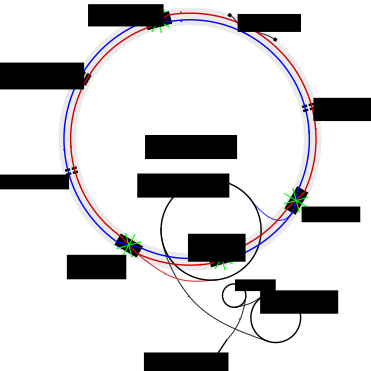
\includegraphics[width=0.8\textwidth]{lhc}
    \caption{Schematic illustration of the \acs{CERN} accelerator complex. Shown are \ac{LINAC} 2, the \ac{PSB}, \ac{PS}, \ac{SPS} and the LHC with its four experiments \acs{CMS}, \acs{ATLAS}, \acs{LHCb} and \acs{ALICE}. The accelerator sizes and positions are not to scale\cite{Ley:CERNAccelerators,Caron:LHCLayout
    ,DeMelis:CERNacceleratorcomplex}.}
    \label{fig:LHC}
\end{figure}

This work will focus on the \ac{CMS} experiment, which will be discussed in the next sections.

\section{The Compact Muon Solenoid}
The \ac{CMS} detector consists of multiple particle detector subsystems surrounding the interaction point.
Its goal is to measure outgoing particles created at proton-proton collisions.
The observed properties include particle type, direction, momentum, energy and charge. Each of the detector subsystems are dedicated to measuring one or more of these characteristics. The subsystems are read out electronically and the data are later analyzed on a computing grid.

An overview of the detector can be seen in \fref{fig:CMS_slice}. The discussion of the detector subsystems in the following sections is based on \cite{Chatrchyan:CMSexperimentCERN} if not explicitly stated otherwise.

\begin{figure}
    \centering
    \raisebox{0.31\height}{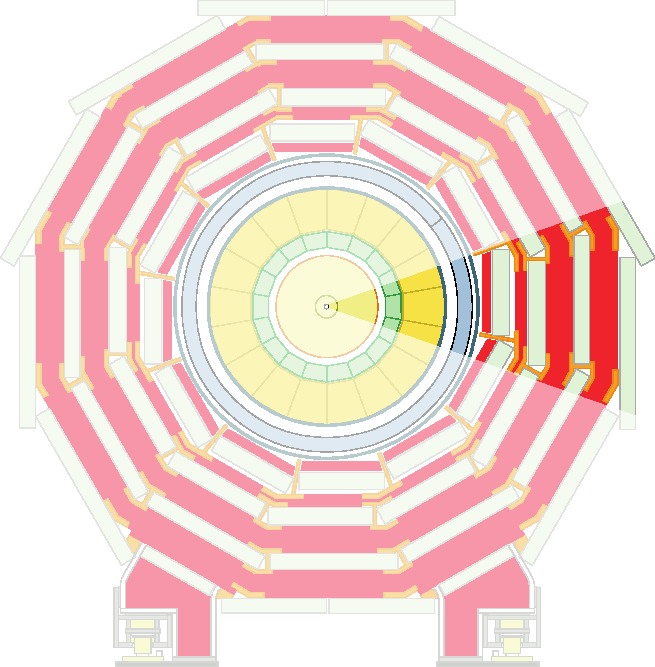
\includegraphics[width=0.3\textwidth]{cms_slice_context}}
    \hspace{0.02\textwidth}
    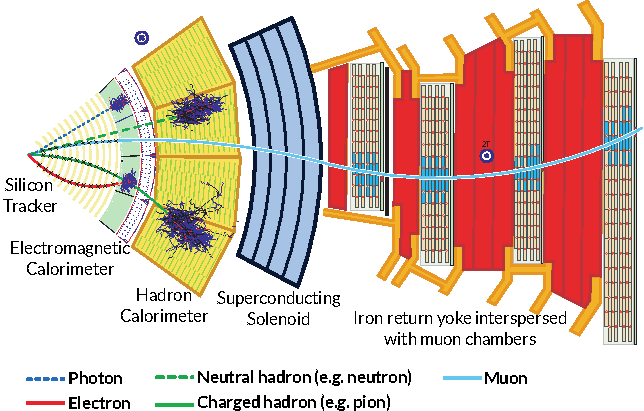
\includegraphics[width=0.65\textwidth]{cms_slice}
    \caption{Slice through the CMS detector barrel. From left to right the following subsystems are drawn: the silicon tracker, the electromagnetic and hadron calorimeter, the superconducting solenoid coil, and the iron return yoke with the muon chambers. The solid lines represent charged particles which are bend due to the magnetic field\cite[modified]{Davis:CMSSlice}.}
    \label{fig:CMS_slice}
\end{figure}

\subsection{Detector Geometry}
In a region starting at \SI{23}{\m} before the detector, both beam pipes are united\cite{Evans:LHCMachine}. The proton groups traveling in opposite directions share the same beam pipe, which defines the $z$-axis of the detector coordinate system. The collisions occur at $z = 0$.
The detector forms a barrel around the beam pipe. The barrel is subdivided into seven slices: five evenly sized \emph{wheels} and one so-called \emph{endcap} on each open side of the barrel. The central wheel is centered at $z = 0$.
Detector layers in the wheels are mostly arranged in a cylindrical manner around the beam pipes, while the layers in the endcaps are mounted orthogonally to the beam pipe.

\subsection{Bunch Crossings and Pile-Up}
\label{sec:pileup}

For acceleration reasons, protons in the \ac{LHC} are grouped into packets called \emph{bunches}. At the interaction point, proton bunches from both directions collide every \SI{25}{\nano\second}, defining the so-called \emph{bunch crossing}. During each bunch crossing, multiple proton pairs may interact with each other. This multitude of collisions is called \emph{pile-up effect}.

Similarly, the collision of a single proton pair may result in multiple partons interacting with each other. This ambiguity is resolved by only analyzing the interaction with the highest momentum transfer, called \emph{hard interaction}. Other interactions contribute to the so-called \emph{underlying event}.

\subsection{Subsystems}
\subsubsection{Inner Tracking System}
The \emph{inner tracking system} is used for precise measurements of direction and curvature of charged particles. 
It is composed of silicon semiconductor pixel layers surrounded by strip modules.

Each pixel cell consists of a silicon semiconductor in reverse bias direction. Charged particles passing through the semiconductor induce ionization and thus allow small currents to flow. These currents are amplified and read out by dedicated electronics. There are about \num{66} million pixel cells, each with a size of $\SI{100}{\micro\meter} \times \SI{150}{\micro\meter}$, allowing for a high spacial resolution.

The strip modules function similarly to the pixel cells. For reduced production costs, typical cell sizes are $\SI{10}{\centi\meter} \times \SI{80}{\micro\meter}$. There are \num{24244} silicon strips in the tracker.

A very high spacial resolution around the interaction point is necessary for finding the origin of decay products. This is achieved by tracing the particle tracks back to the location of their parent particles. The information is later used to discard particle tracks originating in pile-up  events or the underlying event (see \fref{sec:pileup}), as well as for identifying decays of \PB-mesons (see \fref{sec:b_tagging}).

\subsubsection{Electromagnetic Calorimeter}
\label{sec:ecal}
The goal of the \acfi{ECAL} is to measure the energy of outgoing electrons, positrons and photons. 

It consists of dense, transparent lead tungstate ($\textup{PbWO}_4$) crystals. Within these crystals, high energetic electrons and photons cause electromagnetic cascades: Electrons emit photons in the process of bremsstrahlung, while photons convert to electron-positron pairs in the process of pair-production.
This leads to large numbers of lower-energy electrons and photons, until the electron energy loss is dominated by ionization losses and the photon energy is below the pair-production threshold of $2 \si{\electronmass} = \SI{1022}{\keV}$.
Low energetic photons and those emitted by ionization or excitation are eventually registered using photodiodes. The initial particle energy is calculated from the light yield.\cite{ParticleDataGroup:ReviewParticlePhysics}.

As long as the cascade does not leak through the photodetectors, the achieved energy resolution for photons is about \SI{1}{\percent}.\todo{electrons, quelle}

\subsubsection{Hadron Calorimeter}
The \acfi{HCAL} measures the energy of hadrons produced during the collision. 

It is designed as a sampling calorimeter with alternating layers of brass absorbers and plastic scintillator tiles. Hadrons passing through the calorimeter interact with nuclei of the denser brass absorbers. During collisions, secondary charged (\Pgppm, \Pproton, ...) as well as neutral hadrons (\Pgpz, \Peta, ...) are produced. The charged secondaries cause electromagnetic radiation via ionization while the neutral particles decay into photons, which themselves cause electromagnetic showers (see \fref{sec:ecal}).

The charged particles from electromagnetic showers are detected via scintillation. In the plastic scintillators, passage of charged particles induce emission of optical photons. These are guided to photodiodes using wavelength-shifting fibers. The fiber material suppresses Cherenkov light and do not act as scintillators themselves.\cite{ParticleDataGroup:ReviewParticlePhysics}.

Because of the short radiation lengths in the absorber material, sampling calorimeters are more space efficient than homogeneous calorimeters.
However, as some of the energy is deposited within the absorber material, the total shower energy can only be estimated from the scintillation light.

Similarly to the electromagnetic calorimeter, a high resolution can be achieved only as long as the showers do not leak through the calorimeter.

\subsubsection{Solenoid Magnet}
The \ac{CMS} solenoid magnet is designed to deliver a magnetic field strength of \SI{4}{\tesla}. This is achieved by cooling the \SI{220}{\tonne} cold mass to \SI{4.6}{\kelvin}, such that the NbTi wires become superconducting and the current can reach up to \SI{19.5}{\kilo\ampere}.
The magnet surrounds the calorimeters and has a diameter of \SI{6}{\meter}. Within the coil, the magnetic field is approximately uniform with the field lines being parallel to the beam pipe. Outside, the magnetic field lines are closed by an iron yoke, which is interspersed with the muon system.

Particles passing the field are subject to the Lorentz force which subsequently bends their tracks into circular curvatures. This effect allows to distinguish between charged and neutral particles and enables measurement of particle momenta independently of their energy.

\subsubsection{Muon System}
The goal of the muon system is to detect muons and measure their tracks, from which the muon momenta are calculated.

Because of their high mass compared to electrons, muons are less affected by the electromagnetic fields within matter, reducing their radiative losses. This makes them the only detectable particles to pass through all inner detector subsystems as well as the solenoid coil.
For this reason, the muon system is the outermost part of the detector. It surrounds the solenoid coil and consists of \emph{drift tubes} (\acsu{DT}s) and \emph{cathode strip chambers} (\acsu{CSC}s). 

Drift tubes have a length of about \SI{2}{\meter} and a cross section of $\SI{13}{\milli\meter} \times \SI{42}{\milli\meter}$. In the center of each tube, there is an anode wire. Between the wire and the tube walls there is a high electric potential. Additionally, the tubes are filled with a gas mixture. 
As the charged muons pass through the gas, they ionize a few of the gas atoms. The released electrons accelerate along the electric field lines and induce an avalanche of secondary ionizations. Eventually, the accumulated charges are deposited in the anode wires and are measurable as current spike\cite{ParticleDataGroup:ReviewParticlePhysics}.

From the amount of deposited charge and timing measurements, a spacial resolution of less than \SI{250}{\micro\meter} can be achieved across each chamber. However, determining the location in the wire direction is not possible with this arrangement.

In the endcap region, the muon system consists of cathode strip chambers instead of drift tubes. \acp{CSC} work similarly to drift tubes, but instead of having a single cathode at the chamber walls, they contain multiple cathode strips, which are aligned orthogonally to the wires and read out separately.
The advantage of measuring all three dimensions makes them suited for use in the endcap regions where the magnetic field is not uniform. 

\todo{RPCs?}

\subsection{Triggering}
As mentioned in \fref{sec:pileup}, the \ac{LHC} delivers collisions about every \SI{25}{\nano\second}, resulting in around \num{40} million events per second. Even with a raw event size of about \SI{1}{\mega\byte}, storing all events would require a bandwidth of \SI{40}{\tera\byte\per\second}. Currently, there is no technology capable of this task, especially considering the outer circumstances such as irradiation and the strong magnetic field.

Thus, the rate of events accepted for storage and analysis has to be drastically reduced. This is the task of the \emph{triggering system}. Based on the physics content, statistics and bandwidth restrictions, triggers decide whether or not to store an event to disk.

Triggering is implemented in a two step process: First, the \acfi{L1} trigger is consulted. It is implemented in dedicated hardware and uses information from the calorimeters and the muon system to reject low-energetic events. Events passing \ac{L1} will be read out, temporarily stored and further evaluated by the \acfi{HLT}. The \ac{HLT} is implemented in software and running on computers next to the detector cavern. It has access to the full detector information to decide whether an event is eventually stored or rejected.

\subsection{The Computing Grid}
Reconstruction and analyses are ran on the stored events. For this purpose, \ac{CERN} maintains several server farms, organized within the \acfi{WLCG} project.

The facilities are organized in layers called \emph{tiers}. Tier 0 is the \ac{CERN} data center in Geneva. It store raw data and performs initial reconstruction. The data are then distributed to tier 1 computing centers. There are currently 13 tier 1 centers worldwide. They perform further processing on the data and distribute it to tier 3 facilities.

Most of the 155 tier 3 computing centers belong to universities and other scientific institutes. They produce \ac{MC} simulations and perform scientific analyses. One of these tier 3 centers is operated at the physics department of the RWTH Aachen University, currently providing around \num{5200} processing cores and \SI{3}{\peta\byte} of storage. 

\todo{quelle}
% https://home.cern/about/computing/grid-system-tiers
% http://www.institut3b.physik.rwth-aachen.de/cms/ParticlePhysics3B/Forschung/~gbvf/GRID-Computing/


% !TeX spellcheck = en_US
% !TeX encoding = UTF-8
% !TeX root = ../document.tex

\chapter{Model Unspecific Search}

\section{Motivation}
A collision at an energy of \SI{13}{\TeV} can create a large amount of different particles. Solely by combinatorics, it follows that a lot of different final states are accessible.

Most dedicated searches tend to focus on one or a few final states that represent the signature of the theory under investigation. This leaves many final states not examined, either because of the complexity of the final state or because there is no analysis group currently working on a corresponding theory.

One of the goals of the model unspecific search is to gain knowledge from these additional final states. Additionally, the model unspecific search aims to obtain a global interpretation of the agreement between simulation and observed data across a broad range of final states.

\section{Previous Works}
The approach of a model unspecific search is not a new concept: In 1998, a note about an unspecific search has been written at the L3 experiment (\ac{LEP})\cite{Hebbeker:GlobalComparisonL3}, and in 2004, a similar approach has been applied to data of the D0-experiment at the Tevatron proton-antiproton collider at Fermilab\cite{Biallass:ModelIndependentSearch}.

At \ac{CMS}, the analysis has been developed and regularly applied to observed data since 2009\cite{Schmitz:ModelUnspecificSearch,Hof:ImplementationModelIndependent,Dietz-Laursonn:ModelUnspecificSearch,Olschewski:StudyAlternativeStatistical,Brodski:ModelUnspecificSearch,Pieta:MUSiCModelUnspecific,Papacz:ModelUnspecificSearch,Albert:ExtensionModelUnspecific,Roemer:ModelUnspecificSearch} \todo{Jonas' Arbeit, Debby und Simon?}. 
This thesis bases on the most recent implementation of the \ac{MUSiC} analysis.\todo{ok so?}

Very recently, the \ac{ATLAS} collaboration published a conference note analyzing \SI{3.2}{\per\femto\barn} of \ac{LHC} data at $\sqrt{s} = \SI{13}{\TeV}$ using a similar model-independent search \cite{ATLAS:ATLAS-CONF-2017-001}. 

\section{Procedure}
The input to the \ac{MUSiC} analysis are reconstructed events of observed as well as simulated data, which have been centrally reconstructed by the \ac{CMS} collaboration.
As first step of the \ac{MUSiC} analysis, requirements on events and physics objects are applied, discarding unwanted events and extracting objects for the \ac{MUSiC} analysis (see \fref{chap:selection}).
Afterwards, each event is classified sorted into so-called \emph{event classes}, sets of events that share the same final state.
For each event class, the kinematic variables of each event are calculated and \emph{kinematic distributions} are aggregated.
Up to this point, the same procedure is applied to simulated data and observed data.
Subsequently, an automated search algorithms finds the largest deviation between data and simulation within each kinematic distribution of each event class. Afterwards, the global significance of each deviation is estimated from Standard-Model only simulations.

\section{Event Classes}
An event class is a set of events sharing the same final state. The final state is indicated by the name of the event class: All events in the class named \eventclass{2\Pe + 1\Pmu}, for example, contain two electrons and one muon in the final state.

There are three types of event classes: \emph{exclusive}, \emph{inclusive} and \emph{jet inclusive}.

Events in the exclusive event classes contain exactly the indicated (and no additional) particles in their final state. Each event thus belongs to exactly one exclusive event class.

Inclusive event classes are denoted with the suffix "\eventclass{+ X}" in the name (for example \eventclass{2\Pe + 1\Pmu + X}). Their final state contains the explicitly stated particles plus any additional ones. Each event can be assigned any number of inclusive event classes. One advantage of this procedure is a larger number of events per class which can be beneficial \todo{for what?}. However, the correct combination of statistical results across multiple inclusive event classes is not trivial.

Jet inclusive event classes are denoted with the suffix "\eventclass{+ Njets}" in the event class name (e.g. \eventclass{2 \Pe + 1\Pmu + Njets}). Events contained in a jet inclusive event class may contain any number of jets in addition to the explicitly stated objects. This increases the number of events per class, as effects like initial or final state radiation are ignored, leading to reduced statistical uncertainties.

In any case, the kinematic variables are only calculated from the objects explicitly stated in the class name, in our example two electrons and one muon.


\section{Particle Types}
Not all particle types that can be identified by the experiment are used within the classification. Instead, \ac{MUSiC} focuses on a set of five particle types which can be measured most precisely.
Additionally, certain selection criteria are imposed onto each particle in the final state to obtain an unambiguous final state.
The particle types and identification criteria are described in the following sections.

big picture
why ids (why not just reco)
general id criteria: pt, tracks, shower


\subsection{Electrons}



\subsection{Muons}

\subsection{Photons}

\subsection{Jets}

\subsection{Missing Transverse Energy}

\subsection{Possible Extensions}
The analysis can be extended to identify more particle types by their decay products, called \emph{tagging}. Possible tagging choices are \Pqb-tagging, \Ptau-tagging or \PZ-tagging.
This thesis will investigate the increase of sensitivity using \Pqb-tagging. The method is further described in chapter \todo{ref}.

\section{Transverse Momentum and Transverse Energy}
\todo{context?}

Interaction cross sections are often dependent on the amount of momentum involved. In t-channel diagrams, the entire momentum transfer can be measured by calculating the combined invariant mass of decay products.
In order to achieve this goal, one must know all four components of the momentum of all created particles. If the final state contains neutrinos, which are not detectable by the detector, this is not achievable.

In other experiments like \ac{LEP}, one could use conservation of momentum and the known momentum of colliding particles to reconstruct the neutrino four-momentum and the momentum transfer. At the \ac{LHC} this is also impossible: The total proton momentum is distributed unevenly between the constituent quarks and gluons and thus the momentum involved in a collision is only known up to statistical probability.

The mitigation pursued at \ac{CMS} is to only regard kinematics in the transverse plane, orthogonally to the beam pipe. Projection of the kinematic (three-)momentum onto the transverse plane gives the so-called \emph{transverse momentum} \pT.

An additional property of the transverse momentum is that it can be directly observed: Since the magnetic field lines are parallel to the beam direction, the Lorentz force only acts in the transverse plane, allowing direct observation of the transverse momentum.

Assuming $p_x$, $p_y$, $E$ and $m$ can be observed directly (e.g. via track curvature) or indirectly (e.g. via particle identification), we can define the transverse momentum and transverse energy as follows:
\begin{align*}
\vec{p}_T &\defeq \left( p_x, p_y, 0 \right)^T  \\
\vec{E}_T &\defeq E \frac{\vec{p}_T}{\abs{\vec{p}}} = \frac{\vec{p}_T}{\sqrt{1-\left(m/E\right)^2}}
\end{align*}

Note that in the approximation of massless ($m \approx 0$) particles: $\vec{p}_T = \vec{E}_T$. % $ = \vec{M}_T$.

%cross sections are dependent of momentum transfer
%in t-channel diagrams: momentum transfer is invariant mass of created particles
%calculate inv mass from 4-vectors of all particles
%problem if neutrinos are produced
%other approaches (both done at LEP): control COM energy of interaction precisely, or use momentum conservation to reconstruct neutrino 4-momentum
%problem: energy of and initial momentum in beam direction unknown because of partons
%mitigation: use knowledge about momentum in transverse plane, calculate momenta and energy there
%pT has additional advantages: measured directly (magnetic field) and is invariant regarding pdfs/z-boosts

\section{Kinematic Variables and Distributions}
For each event, the \ac{MUSiC} classification calculates three scalar variables: the sum of transverse momenta, the invariant mass and the missing transverse energy.

The sum of transverse momenta is the most directly observed variable. For charged particles, the transverse momentum can be deduced directly from the curvature within the magnetic field. The transverse momentum is invariant against Lorentz-boosts in the $z$-direction from the uneven momentum distribution within the proton.
In the following, the sum of transverse momenta will be denoted with \sumpT and defined as follows:
\begin{equation}
    \sumpT \defeq \sum_i \abs{\vec{p}_{T,i}} 
\end{equation}

The invariant mass is, as mentioned before, very sensitive to resonances in the t-channel. If the event class definition contains missing transversal energy passing the selection criteria, the invariant mass will not be computed, instead the transversal mass is used. The variables are denoted with \Minv and \MT respectively and defined as:
\begin{align}
    \Minv &\defeq \sqrt{\left(\sum_i E_i\right)^2 - \left(\sum_i \vec{p}_i\right)^2} \\
    \MT &\defeq \sqrt{\left(\sum_i E_{T,i}\right)^2 - \left(\sum_i \vec{p}_{T,i}\right)^2}     
\end{align}

The third kinematic variable is missing transversal energy. This variable is only calculated if the event class definition explicitly contains missing transversal energy.
The variable is denoted with \MET defined as follows:
\begin{equation}
    \MET \defeq \abs{- \sum_i \vec{E}_{T,i}} 
\end{equation}


\section{Search for Deviations}
\label{sec:deviations_search}

\newcommand{\TS}{\ensuremath{\uptheta}\xspace}
\newcommand{\TSmin}{\ensuremath{\theta_\text{min}}\xspace}

After the classification follows an automated search for deviations. The search is performed on each distribution of each event class separately as follows:
First, multiple bins are combined to a \emph{region}, according to the rules in the following section. Then, a test statistic \TS for each region is calculated. The region with the lowest value of \TS, called \TSmin, is selected. This region will be called \acfi{RoI}. 
Subsequently, a global $\ptilde$-value for the region is calculated. This $\ptilde$-value expresses the probability of finding a deviation with $\TS \leq \TSmin$ purely by chance. Details on the procedure can be found in \fref{sec:global_significance}.

\subsection{Search Space}
The search is performed on so-called regions. A region is a set of adjacent bins and is represented by the combined number of expected and observed events as well as a combined uncertainty.

For the \sumpT and \MET kinematic distributions, the minimal number of bins in a region is \num{3}, in order to be insensitive towards narrow deviations from \ac{MC} statistics \todo{explain spikes}.
For a increased sensitivity to resonant deviations, the minimal number of bins in the \Minv and \MT distributions is \num{1}.

An additional criterion on the regions is based on the number of simulated events in a region. If a region shows a lack of simulated events, the test statistic is not computed for this particular region. Since each region (that is not the entire distribution) is embedded in a larger region, regions skipped in this step are still considered. \todo{low stats ausfuerlicher erklaeren?}

The combined number of events and the combined uncertainty for each region is calculated as
\begin{align}
     N_{\text{total},\text{exp}} &= \sum_i N_{i, \text{exp}} \\   
     N_{\text{total},\text{obs}} &= \sum_i N_{i, \text{obs}} \\
     \sigma_\text{total} &= \sqrt{\sum_i \sigma_i^2 + 2 \sum_{i,j} \rho_{i,j}\sigma_i\sigma_j}
\end{align}
where $\rho_{i,j}$ is the correlation coefficient for the uncertainty $\sigma$ between the bins $i$ and $j$.

Some uncertainties, such as the statistical uncertainty on the simulated number of events, are completely uncorrelated between the bins. The correlation coefficient thus is $\rho_{i,j} = 0$ and the total uncertainty is the quadratic sum of the bin uncertainties.

Other uncertainties are correlated between bins. An example for this is the uncertainty on the luminosity measurement, which affects all bins of all distributions the same way. We treat any uncertainty that is assumed to be correlated to some extend as fully correlated ($\rho_{i,j} = 1$) and calculate the combined uncertainty as linear sum. This method possibly overestimates the total uncertainty, in case the correlation coefficient is somewhere between 0 and 1, leading to a lower \todo{(conservative?)} sensitivity.

\subsection{Global Significance}
\label{sec:global_significance}

The goal of the automated search is to find the largest deviation between expected and observed number of events in a region. The size of a deviation is expressed as value of the test statistic \TS. A larger deviation will result in a smaller value of \TS.
The formula for computing \TS will be derived in the next chapter. \todo{mention \TS = local p value?}

From the test statistic, we will calculate a global significance, to which we refer as \ptilde. It expresses the probability of finding a deviation equally large or larger than the observed one somewhere in the distribution, if the expectation were true.

The simplest way of calculating \ptilde would be to first calculate a local $p$-value from the test statistic and then apply a correction factor to it. A suitable correction factor can be estimated using combinatorics, if the possible values of the local $p$-value are uncorrelated. This method is also called \emph{Bonferroni correction}. 

In our case, a purely analytically calculation is not possible because the connected bin regions overlap and thus the local significances are correlated.

Instead, we use a simulation-based approach:
We simulate possible experimental outcomes based on the distribution of expected number of events, and refer to each simulation round as \emph{pseudo-experiment}.
During each pseudo-experiment, we randomly draw a substitute observed distribution from the expected number of events. 

correlated uncerts: shared value of standard gaussian multiplied with local width of uncert
uncorrelated: random from normal distribution
summed up
poissonian draw for quantum-phenomena

\begin{algorithm}
    \caption{Pseudo Experiment}
    \newcommand{\Nobs}{n}
    \newcommand{\Nexp}{N}
    \newcommand{\corr}{corr}    
    \newcommand{\uncorr}{uncorr}
    \newcommand{\x}{x}
        
    \begin{algorithmic}
        \Require $\Nexp_{i=1..n} \gets $ number of events in each bin $i$
        \Require $\corr_{i=1..n,j=0..c} \gets $ correlated uncertainty $j$ in each bin $i$
        \Require $\uncorr_{i=1..n,k=0..u} \gets $ uncorrelated uncertainty $j$ in each bin $i$
        
        \Statex
        
        \ForAll {correlated uncertainty $j$ in distribution}
            \State $\x_j \gets \text{RandNormal}(\mu = 0, \sigma = 1)$
        \EndFor
        
        \ForAll {bin $i$ in distribution}
            \State $\Nobs_i \gets \Nexp_i$
            \ForAll {correlated uncertainty $j$ in bin $i$}
                \State $\Nobs_i \gets \Nobs_i + \x_j \cdot \corr_{i,j}$
            \EndFor
            \ForAll {uncorrelated uncertainty $k$ in bin $i$}
                \State $\Nobs_i \gets \Nobs_i + \text{RandNormal}(\mu = 0, \sigma = \uncorr_{i,k})$
            \EndFor
            \State $\Nobs_i \gets \text{RandPoisson}(\Nobs_i)$
        \EndFor
    \end{algorithmic}
\end{algorithm}

The recipe for each pseudo-experiment is as follows:

Let $\sigma_u(i,j)$ be the value of the uncorrelated uncertainty and $\sigma_v(i,j)$ the value of a correlated uncertainty with index $j$ in bin $i$. Further, let $\ev{N_{i}}$ be the expected number of events in bin $i$.



Start by simulating a pseudo-true value for correlated uncertainties since this impacts all bins differently, we choose from a standard normal distribution $\mathcal{N}$:
\begin{equation}
    v_j \sim \mathcal{N}(\mu = 0, \sigma = 1)
\end{equation}

The impact factor for uncorrelated uncertainties is calculated separately for each bin:
\begin{equation}
    u_{i,j} \sim \mathcal{N}(\mu = 0, \sigma = 1) 
\end{equation}

\begin{equation}
    \ev{n_i} = \ev{N_i} + \sum_j^{\text{uncorrelated}} u_{i,k} \sigma_u(i,j) + \sum_k^{\text{correlated}} v_{i,k} \sigma_v(i,k)
\end{equation}

Finally draw an integer value from the Poisson distribution $\mathcal{P}$ with the expectation value $\ev{n_i}$.
\begin{equation}
    n_\text{obs} \sim \mathcal{P}(\lambda = \ev{n_i})
\end{equation}


For each \emph{pseudo-experiment}, we draw a random number of events for each bin of the distribution simultaneously. The number is drawn from the probability distribution caused by systematical and statistical uncertainty around \ac{SM} expectation value. 


 of \emph{pseudo-experiments}: For each bin of the distribution, a random number is drawn from the probability distribution caused by systematical and statistical uncertainty on the \ac{SM} expectation value. The resulting \emph{pseudo-distribution} is subsequently again compared to the expectation using the described search algorithm, yielding a local significance value \TS for each pseudo-experiment.
The step of randomly generating a distribution and searching for a deviation is repeated \num{e5} to \num{e6} \todo{number} times.

Finally, the global \ptilde-value is calculated by determining the rate of pseudo-experiments where $\TS_{\text{random}, \text{min}} < \TS_{\text{obs}, \text{min}}$. Note that the definition of a $p$-value ("probability to find a deviation equally large or larger as the observed one by chance") corresponds directly to the computed \ptilde-value in the frequentist interpretation.

%Within the (statistical and systematical) uncertainty distribution of the Standard Model  
%The statistical nature of the Standard-Model is simulated by randomly choosing values for the observed number of events in each bin.
%The probabilities of observing deviations are correlated between overlapping regions. 
%Since the regions' overlap, the regions are correlated. Thus, the probabilities of observing deviations by chance are correlated between overlapping regions.
%assess the significance of a deviation, expressed as probability to observe a deviation the same as or more extreme just by chance (given SM) SOMEWHERE in the distribution
%procedure also known as Bonferroni correction
%correction factor cannot be calculated analytically because of correlations between regions
%idea: pseudo-experiment, simulate circumstances using SM only, count more-extreme values, interpret fraction as probability (frequentist  approach)
%problem: need measure for "extremity" of deviation (-> also used for finding RoI)

\subsection{Test Statistic}
\label{sec:test_statistic}

measure "extremity" of deviation (-> for finding RoI as well as global correction)

choice is ambiguous

choice: value interpretable as probability for local deviation

back to definition: sum of probabilities of more extreme events

start using Poissonian probability
include Gaussian prior: either normal or log normal


most of the systematic uncertainties scale number of events in a region rather than a constant shift. examples: lumi, xsec, PDF, ID efficiency, misID


The total number of events is thus scaled by an unknown factor $X$, which is a random variable that emerges as product of multiple other random variables $x_i$.
In the following section, we will derive how $X$ is distributed.

We begin with rewriting the product in terms of a sum within an exponential distribution:
\begin{equation}
    X = \prod_i x_i = \prod_i \exp(\ln(x_i)) = \exp(\sum_i \ln(x_i))
\end{equation}
$\ln(x_i)$ is a random variable, and the central limit theorem implies that the sum is distributed according to the normal distribution.
\begin{equation}
    Y \defeq \sum_i \ln(x_i) \Rightarrow X = \exp(Y) \text{ and } f_Y(y) = \frac{1}{\sqrt{2\pi}\sigma} \exp(-\frac{1}{2}\left(\frac{y-\mu}{\sigma}\right)^2)
\end{equation}
After defining $Y$ as the normally distributed variable with the probability density $f_Y(y)$, we introduce a new unknown probability density function $g_X(x)$:
\begin{equation}
    f_Y(y) \: \dd y \eqdef g_X(x) \: \dd x 
\end{equation}
Finally, we can insert all definitions, calculate the derivative and write the distribution function dependent of $x$:
\begin{align}
    g_X(x) &= f_Y(y) \: \dv{y}{x} \\
    &= f_Y(\ln{x}) \: \dv{\ln{x}}{x} \\
    &= f_Y(\ln{x}) \: \frac{1}{\abs{x}} \\
    &= \frac{1}{\sqrt{2\pi}\sigma\abs{x}} \exp(-\frac{1}{2}\left(\frac{\ln{x}-\mu}{\sigma}\right)^2)
\end{align}
The result is known as \emph{log-normal distribution} and is the probability density function of a product of random variables.

By performing two substitutions, we obtain a parametrization with a more meaningful interpretation:
\begin{equation}
    \sigma \rightarrow \ln{k} \text{ and } \mu \rightarrow \ln{x_0}
\end{equation}
\begin{equation}
    g_X(x) = \frac{1}{\sqrt{2\pi}\abs{x}\ln{k}} \exp(-\frac{1}{2}\left(\frac{\ln(x/x_0)}{\ln{k}}\right)^2)
\end{equation}

\todo{explain meaning of parameters}

\subsection{Treatment of Regions With Too Few Simulated Events}


\subsection{Look-Elsewhere-Effects}
\subsubsection{Regions}
corrected using global significance 

\subsubsection{Classes}
\subsubsection{Distributions}

\section{Implementation}
\subsection{Software Environment}
CMSSW, ROOT, Python/C++

\subsection{Analysis Framework}
Skimming, Pxl, TAPAS, MUSiC

\subsection{MUSiC Workflow}

\subsection{Automation}
\begin{figure}
    \centering
    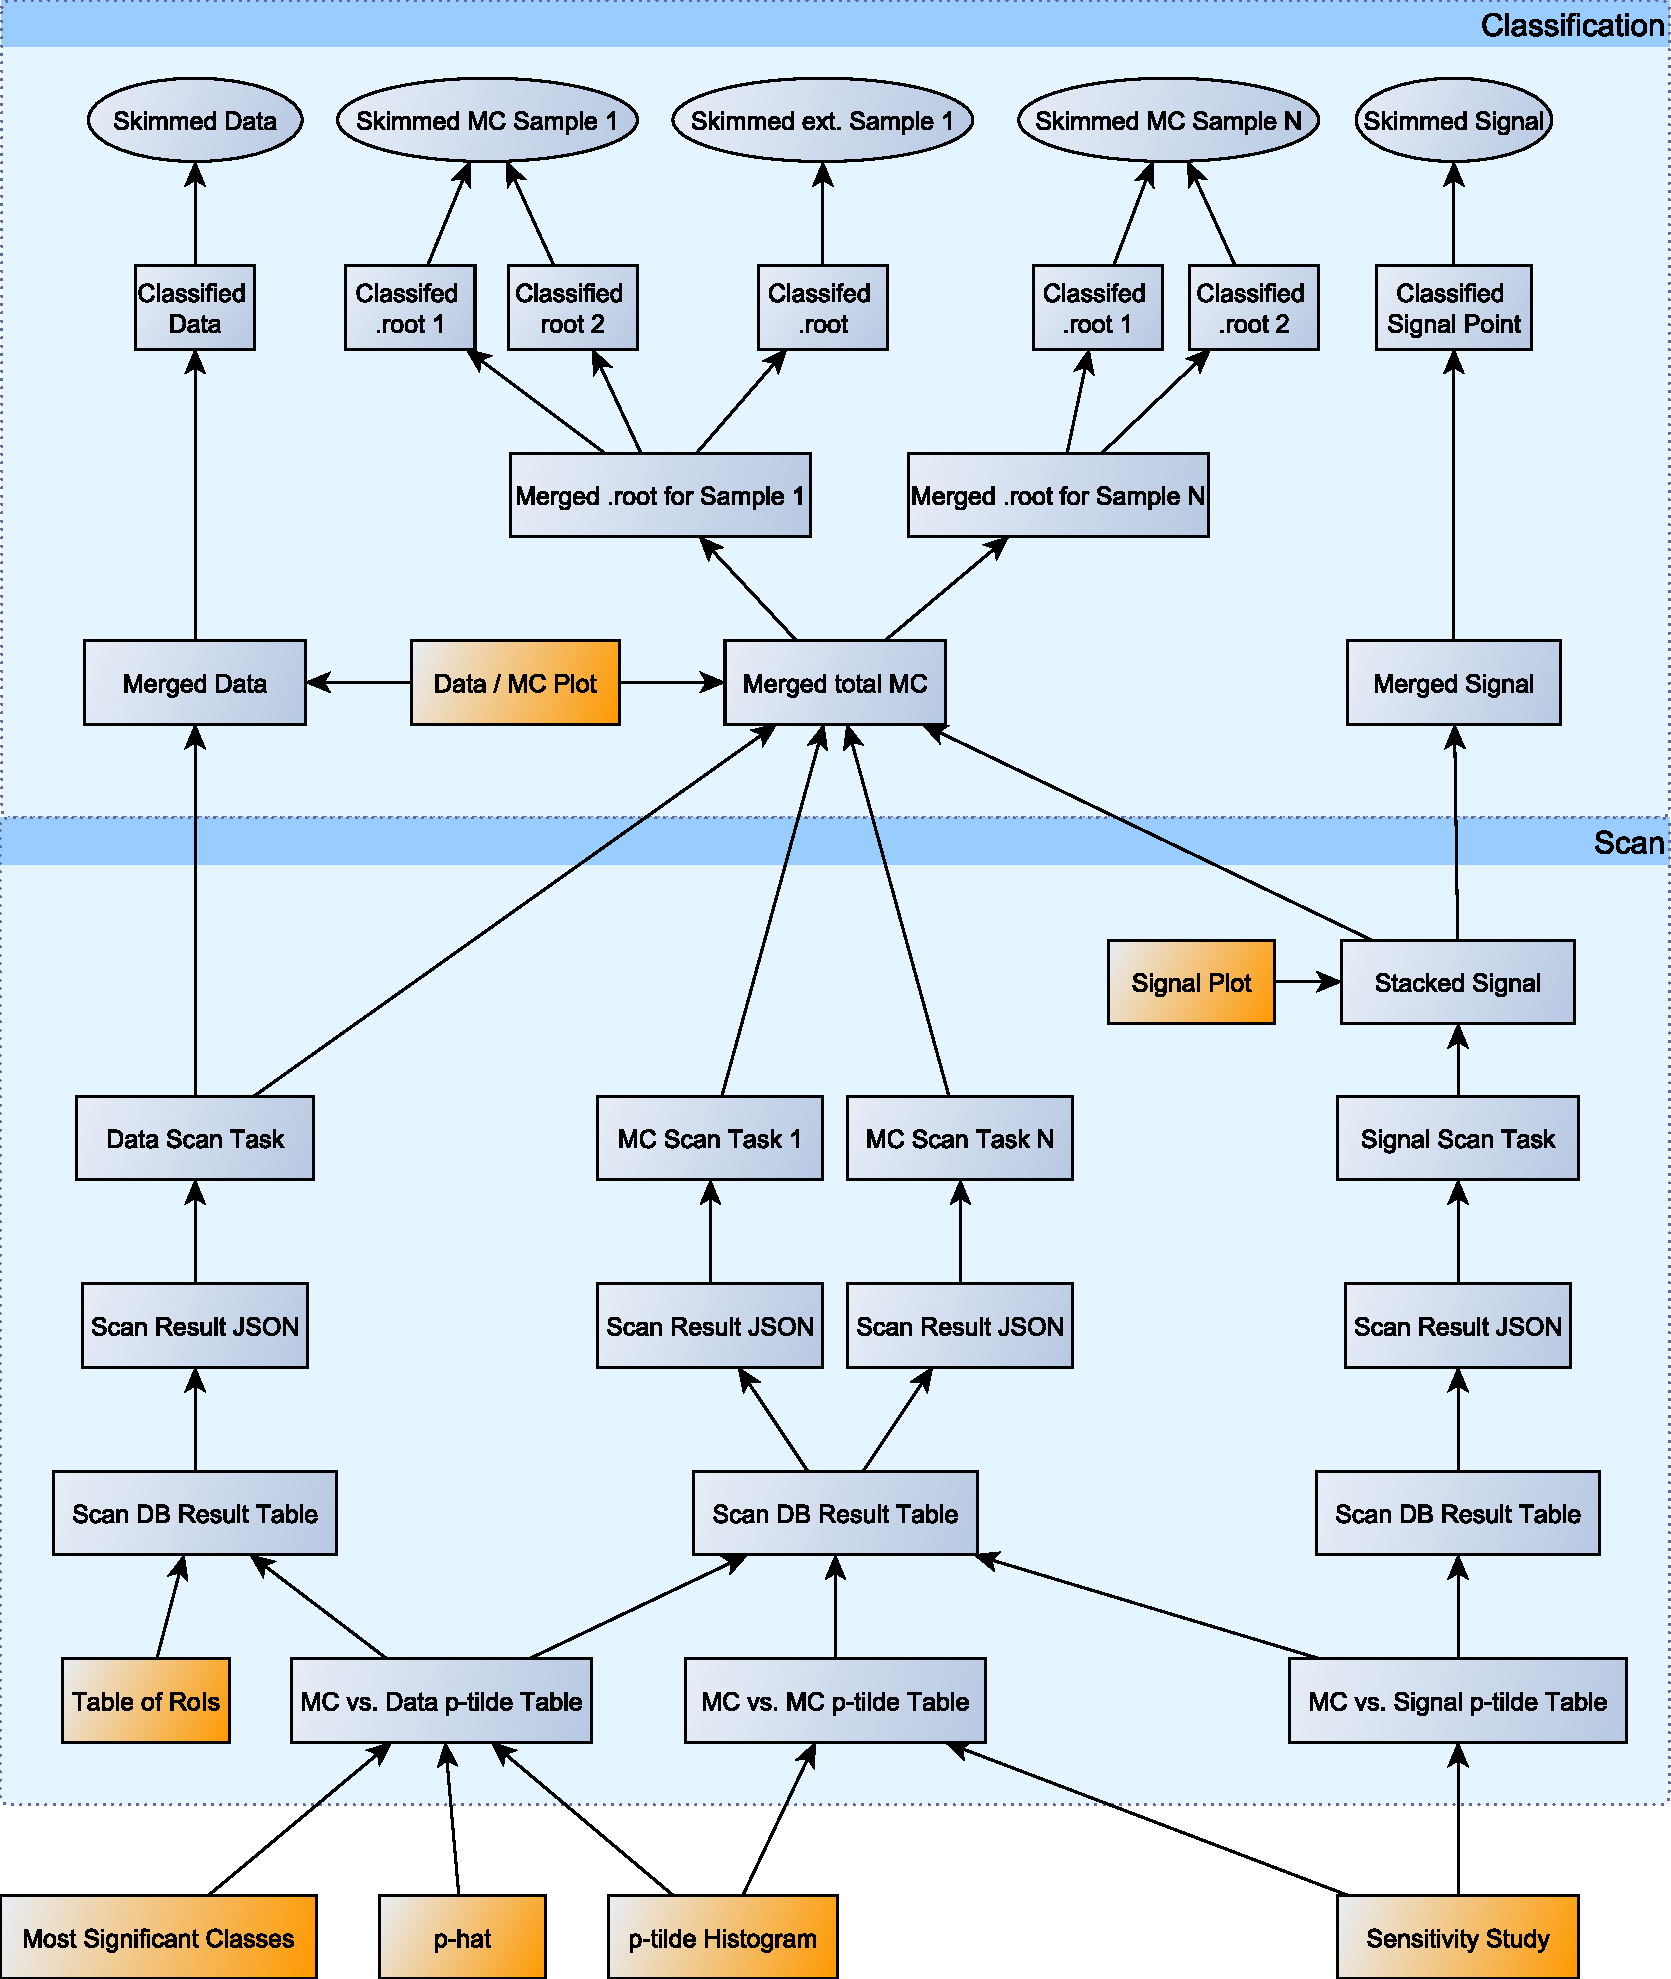
\includegraphics[width=\textwidth]{../music-workflow}
    \vspace{0.5em}
    \caption{Implementation of the MUSiC-Workflow. Using the Luigi-Automation Framework, these steps are performed on demand.}
    \label{fig:music_workflow}
\end{figure}

Luigi
% !TeX spellcheck = en_US
% !TeX encoding = UTF-8
% !TeX root = ../document.tex

\chapter{Datasets}
\section{Monte-Carlo Simulations}
The \ac{MUSiC} analysis aims to search for deviations in a large number of final states and a wide kinematic phase space. Deviations are expected in any area under investigation and therefore there is no signal-free region that could be used for validation or fine tuning. Thus, we avoid data-driven methods as much as possible and rely on theoretical predictions in form of \acl{MC} simulations.

The \ac{MC} simulation is performed on an event-by-event basis. Each event is generated in multiple steps: First, the distribution of proton momentum between partons is simulated. This is done by drawing pseudo-random numbers according to probability distributions related to the empirically measured \emph{parton density functions}.
Afterwards, the hard scattering process is simulated. Similarly as with the momentum distribution, different scenarios are are possible, each with a probability corresponding to the predicted scattering probability. In the second step, parton showering and hadronization is applied: Since the required higher order terms of \ac{QCD} cannot be computed exactly, several parametrized models are used to simulate the formation of hadrons from quarks and gluons. In the last step, the detector response is simulated, also using parametrized interactions of the final state particles with detector components.

In practice, events of different physics processes are simulated in separate sets, so-called \emph{samples}. 
Additionally, some samples only contain events within a certain \pT or mass range. This is done in order to provide a low statistical uncertainty in the tails of steeply falling distributions.

In order to have consistent and validated samples for all \ac{CMS} analyses, the \ac{MC} samples are generated centrally by \ac{CMS} on the \ac{WLCG}.

In addition to weight assigned by generators, each event is assigned a further weight during the analysis. It is computed from the expected cross section, an expected higher order correction factor ($k$-factor) and the luminosity. 
Additionally, events are reweighted to compensate for difference pileup simulation between expectation and data. 
The expected event yield with certain properties can now be obtained by summing the weights of the desired events.

Within this thesis, various luminosity scenarios are analyzed. We did not generate additional \ac{MC} events for each scenario, instead the events are scaled to the described luminosity with the method mentioned above. This allows for a direct comparison ignoring hardware changes made to the detector between the data taking periods in 2015 and 2016.


\subsection{Standard Model}

\newcommand{\genAM}{\textsc{MadGraph\_aMC@NLO}\xspace}
\newcommand{\genBM}{\textsc{BlackMax}\xspace}
\newcommand{\genCA}{\textsc{CalcHEP}\xspace}
\newcommand{\genMG}{\textsc{MadGraph~5}\xspace}
\newcommand{\genPH}{\textsc{Powheg}\xspace}
\newcommand{\genPY}{\textsc{Pythia~8}\xspace}
\newcommand{\genQBH}{\textsc{QBH~2.0}\xspace}
\newcommand{\genSP}{\textsc{Sherpa}\xspace}
\newcommand{\genMCFM}{\textsc{MCFM}\xspace}

\newcommand{\genGEANT}{Geant~4\xspace}

The \ac{SM} samples used by \ac{MUSiC} are produced with the following generator applications: \genMG\cite{Alwall:MadGraph5}, \genSP\cite{Gleisberg:EventgenerationSHERPA}, \genPH\cite{Frixione:MatchingNLOQCDa,Alioli:generalframeworkimplementing}, \genAM\cite{Alwall:automatedcomputationtreea}, \genMCFM\cite{Campbell:Vectorbosonpaira} and \genPY\cite{Sjoestrand:BriefIntroductionPYTHIA}. For the generators \genMG, \genPH, \genAM and \genMCFM, the subsequent hadronization is applied separately using \genPY.
The detector response is simulated with \genGEANT \cite{Agostinelli:GEANT4asimulationtoolkit}.

The full list of used \ac{MC} samples can be found in \fref{app:mc_datasets}.

\subsection{Signal Samples}
The signal study uses the same set of signal samples as the corresponding dedicated analyses \cite{CMS:CMS-PAS-EXO-16-001,CMS:CMS-PAS-EXO-15-007,CMS:CMS-PAS-EXO-16-002,CMSCollaboration:SearchesWbosons}. This makes results comparable and also allows reusing central production and reconstruction by \ac{CMS}. The mass points are chosen to cover a broad range including the resulting limits set by the dedicated analyses. However, since the automated search has to be re-run for each signal sample, computation time limits the amount of samples analyzed.
\begin{itemize}
    \item For the \ac{QBH} model, the \acf{ADD} model with $n = 4$ extra dimensions is analyzed. The chosen mass points $M$ are \SI{1}{\TeV}, \SI{2}{\TeV}, \SI{3}{\TeV}, \SI{4}{\TeV} and \SI{5}{\TeV}. The events are simulated by the \genQBH\cite{Gingrich:MonteCarloevent} generator.
    
    \item In the black hole study, we consider the case of a non-rotating black hole. The fundamental Planck mass is set to $M_\text{D} = \SI{4}{\TeV}$ with $n = 6$ extra dimensions. This choice corresponds to the benchmark result published in \cite{CMS:CMS-PAS-EXO-15-007}. The black hole mass is varied between \SI{6}{\TeV}, \SI{7}{\TeV}, \SI{8}{\TeV}, \SI{9}{\TeV}, \SI{10}{\TeV}. The \ac{MC} generator used for the model is \genBM\cite{Dai:BlackMaxblackhole}.
    
    \item For the Seesaw-TypeIII samples, only the mass points $M_\Sigma = \SI{380}{\GeV}$ and $M_\Sigma = \SI{500}{\GeV}$  are tested. The samples are generated with \genAM\cite{Alwall:automatedcomputationtreea}.
    
    \item The \PWprime model is tested for \PWprime masses of \SI{3}{\TeV}, \SI{4}{\TeV}, \SI{5}{\TeV}. The branching ratio of $\PWprime \to \Ptop \Pbottom$ is set to 1. This sample uses the \genCA\cite{Belyaev:CalcHEP34collider} generator.
\end{itemize}
Again, where necessary, hadronization is applied using \genPY and the detector response is simulated with \genGEANT.

% !TeX spellcheck = en_US
% !TeX encoding = UTF-8
% !TeX root = ../document.tex

\newcommand{\TSprime}{\ensuremath{\TS_\text{LN}}\xspace}
\newcommand{\sigmatrue}{\ensuremath{\sigma_\text{true}}\xspace}

\chapter{Additional Studies}
\section{Coverage Analysis}
\label{sec:coverage}

In this chapter, we will show that the test statistic \TS introduced in \fref{sec:test_statistic} can be directly interpreted as $p$-value: $p = \TS$. We will refer to the definition and requirements of a $p$-value and show that \TS sufficiently fulfills those requirements.
Additionally, we will repeat the analysis with \TSprime, using the log-normal prior (as used in previous \acs{MUSiC} theses) instead of the normal term in \TS and compare the results.

A $p$-value is an indicator for the significance of a deviation, where a smaller $p$-value corresponds to a higher significance. The $p$-value of a result is compared to a significance threshold $\alpha$, which is fixed before the statistical analysis. If the observed $p$-value is smaller than $\alpha$, the null hypothesis is rejected. In our case, rejection of the null hypothesis corresponds to falsification of the \acl{SM} and thus the discovery of new physics. 

Both values are constructed in way that the null hypothesis is (incorrectly) rejected by chance with a probability of $\alpha$:
\begin{align}
	\Pr( H_0\:\text{rejected} | H_0 ) &= \alpha \\
    \label{eq:coverage_inequality}
    \Rightarrow \Pr( p < \alpha | H_0 ) &= \alpha
\end{align}
This equation is tested during the \emph{coverage analysis}.

\subsection{Procedure}
To test \fref{eq:coverage_inequality}, we construct pseudo experiments based on the null hypothesis $H_0$ and calculate the corresponding $p$-value, in this case \TS or \TSprime. After generating and examining sufficiently many pseudo experiments, we can determine the rate of significant findings and compare them to the claimed significance threshold:
\begin{equation}
	p_\text{true} = \frac{\text{number of pseudo-experiments where $p < \alpha$}}{n_\text{toys}} = \Pr(p < \alpha | H_0)
    \label{eq:coverage}
\end{equation}

The pseudo experiments are based on \acs{MUSiC}'s null hypothesis: 
We assume that there is a constant probability that events end up in a particular region, and thus a constant true mean value \Ntrue. 
We also assume that this true mean value is only known up to an expected event yield, \Nmc.
The way that \Nmc is derived from \Ntrue differs between \TS and \TSprime: For \TS, \Nmc is drawn from a normal probability density, \TSprime  will use a log-normal distribution instead.

Additionally, the physics process of performing a counting experiment has to be simulated: Here it is assumed that the event yield is caused by independent statistical processes with a fixed probability, thus the observed event yield follows a Poisson distribution around \Ntrue.

The way that the assumed uncertainty enters the pseudo experiment also differs between \TS and \TSprime: For \TS, the absolute uncertainty is kept constant: $\sigmamc = \sigmatrue$. For \TSprime, we recalculate the uncertainty after drawing \Nmc in order to keep the relative uncertainty constant: $\sigmamc = \frac{\Nmc}{\Ntrue} \sigmatrue$.
This has been discussed by \cite[p. 78]{Schmitz:ModelUnspecificSearch}, a more rigorous discussion can be found in \fref{app:coverage_uncertainty}.

In the implementation, each pseudo-experiments begins with drawing \Nmc from the probability density around \Ntrue. At the same time, \Ndata is drawn from a (discrete) Poisson distribution with a mean of \Ntrue. From these two values, as well as the uncertainty \sigmamc, \TS (or \TSprime) is calculated.

This process is repeated for $n_\text{toys}$ pseudo-experiments. An estimation for the true $p$ value is afterwards calculated using \fref{eq:coverage}, which yields the left hand side of \fref{eq:coverage_inequality}.

In order to state the so called "coverage value" for the tuple (\Ntrue, \sigmatrue), both sides of  \fref{eq:coverage_inequality} are translated to $Z$-scores (see \fref{app:z_score}), resulting in $Z_\text{true} = Z(p_\text{true})$ representing the observed and $Z_\text{claim} = Z(\alpha)$ representing the claimed rate ob significant results.
The coverage is finally reported as
\begin{equation}
    \label{eq:coverage_value}
	\text{coverage} = Z_\text{true} - Z_\text{claim}.
\end{equation}
%or alternatively as 
%\begin{equation}
%    \text{coverage}' = \log_{10} %\left(\frac{p_\text{true}}{p_\text{claim}}\right)
%\end{equation}

\subsection{Interpretation of Results}
Three different result cases can arise, depending on the coverage value in \fref{eq:coverage_value}:
\begin{enumerate}
	\item $\text{coverage} = 0 \Leftrightarrow \Pr( H_0 \text{ rejected} | H_0 ) = \alpha$: This is the ideal case. It indicates the $p$-value performs according to its definition.
	\item $\text{coverage} < 0 \Leftrightarrow \Pr( H_0 \text{ rejected} | H_0 ) > \alpha$: The background hypothesis is rejected more often than with a probability of $\alpha$. This case is called "undercoverage" and corresponds to "liberal" behavior. The $p$-value overestimates the significance of deviations.
	\item $\text{coverage} > 0 \Leftrightarrow \Pr( H_0 \text{ rejected} | H_0 ) < \alpha$: The background hypothesis is not rejected in some cases where it should have been rejected. This effect is called "overcoverage" and corresponds to "conservative" behavior where the $p$-value underestimates the significance of deviations.
\end{enumerate}	

\subsection{Our Results}
Since the MUSiC $p$-value is required to cover a large range of possible \Ntrue and relative uncertainty $\sigmatrue / \Ntrue$ values, the coverage is evaluated on a two dimensional grid in this parameter space.
The computed results for \TS can be found in \fref{fig:coverage_normal}, for \TSprime in \fref{fig:coverage_lognormal}. 

\begin{figure}
    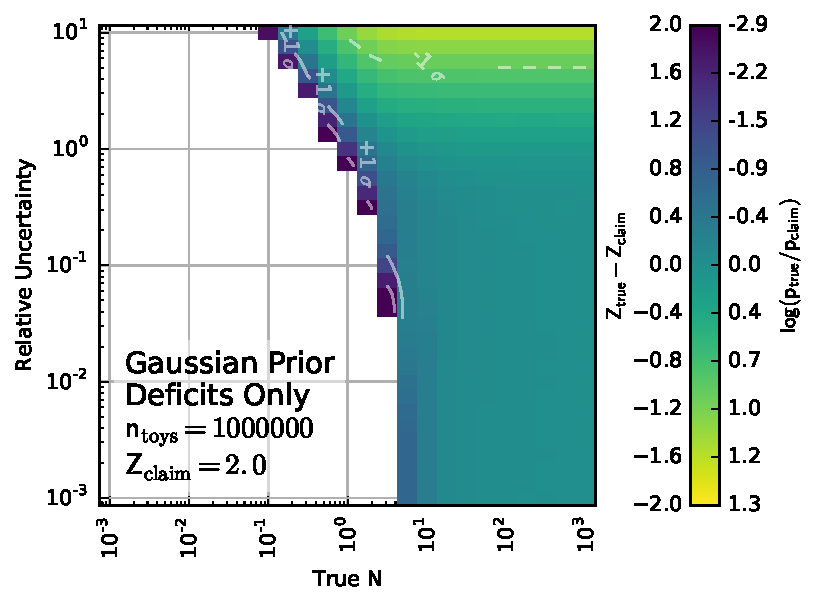
\includegraphics[width=\textwidth]{coverage/coverage_deficit_normal_log}
    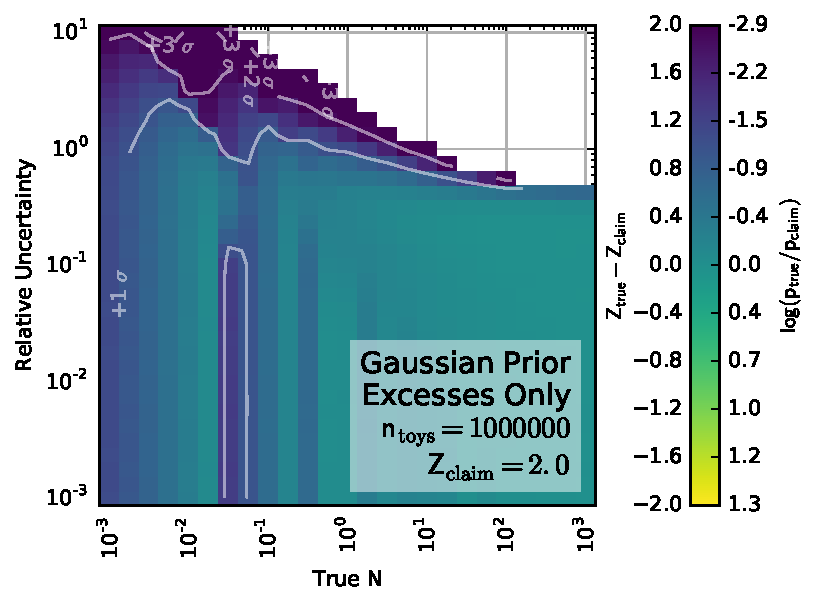
\includegraphics[width=\textwidth]{coverage/coverage_excess_normal_log}
    \caption{Results of the coverage analysis for \TS, using the Gaussian prior. The figure on top shows that coverage for deficits, the bottom figure indicates coverage behavior for excesses. Within the blank areas, the coverage value could not be determined since no significant result could be observed.}
    \label{fig:coverage_normal}
\end{figure}

\begin{figure}
    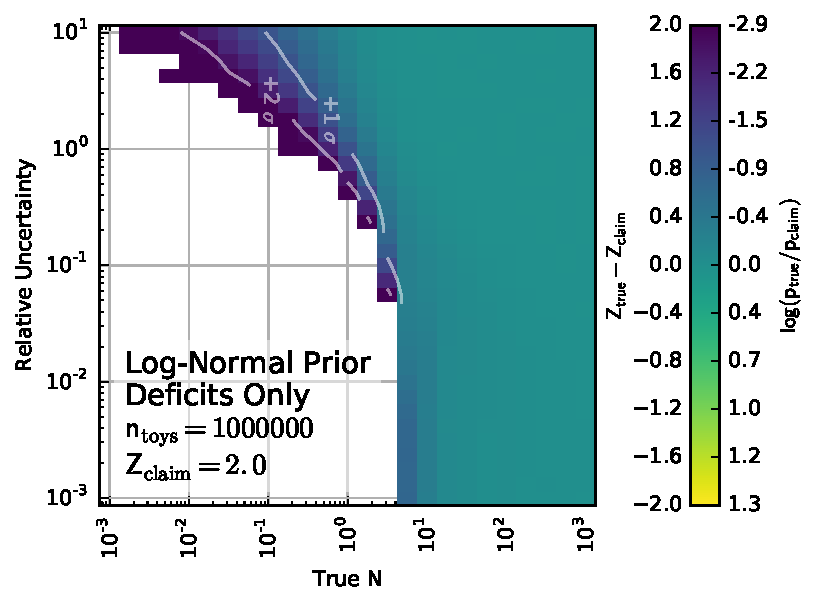
\includegraphics[width=\textwidth]{coverage/coverage_deficit_lognormal_log}
    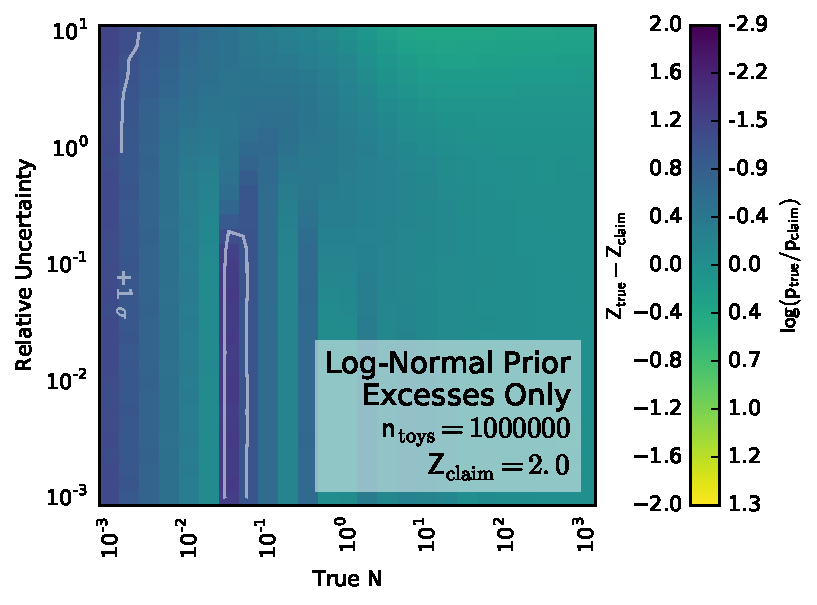
\includegraphics[width=\textwidth]{coverage/coverage_excess_lognormal_log}
    \caption{Results of the coverage analysis for \TSprime, using the log-normal prior. The figure on top shows that coverage for deficits, the bottom figure indicates coverage behavior for excesses.}
    \label{fig:coverage_lognormal}
\end{figure}

Areas tinted with dark blue color have determined to be overcovered (conservative behavior), while the bright yellow shows areas of undercoverage. Within the blank areas, the coverage value could not be determined since no significant result could be observed. This is expected, especially for deficits below $\Ntrue = \num{1}$, because at $\Nmc < \num{1}$, the only possible deficit is $\Ndata = \num{0}$, which is not significant ($p = \num{0.37}$ with $\sigmamc \rightarrow \num{0}$).

Further illustrations in non-logarithmic view can be found in \fref{app:coverage_additional_results}.

\subsubsection{Results for \TS}
For the Gaussian prior in \TS, one can see almost ideal coverage for $\Ntrue > \num{1}$ and $\sigmamc/\Ntrue < \SI{50}{\percent}$. This is compatible with the results from earlier studies\cite{Schmitz:ModelUnspecificSearch}, which have partially been reproduced in \ref{app:coverage_schmitz}.

In both cases (deficits and excesses), the coverage value gets worse at high relative uncertainties. This is due to the truncation of the normal distribution at \num{0}. In the excess case, the conservativeness prevents any significant results to appear during the coverage study, therefore the area stays blank.

\todo{versuchen zu erklären, warum?}

% excess, uncert -> inf => p->1

% deficit, uncert -> inf => p->0 siehe Script truncated_normal
% C -> linear in \sigma, integral -> 1 ==> p = ratio -> 0

\subsubsection{Results for \TSprime}
The log-normal prior shows much better coverage values across the probed range. There are areas of slight overcoverage, but especially in the excess case the overcoverage does not exceed $\num{1} \sigma$.


\section{Log-Normal $p$-Value}
\label{sec:lognormal_pvalue}

As observed in the previous section, using the truncated normal distribution as prior within the $p$-value has limited validity at high relative uncertainties.
At the same time, we have observed that using a log-normal prior improves test coverage in the problematic regions.

In addition, a log-normal prior is more suited for modeling our uncertainties: Analogously to the normal distribution, which is generated from a sum of independent random variables, the log-normal distribution results from the multiplication of independent random variables (see \fref{app:lognormal_derivation}). The latter corresponds to our situation, as most uncertainties on the event yield originate from shifting the event yield by a multiplicative factor.
Also note that in the limit of $\Nmc \rightarrow \infty$ and $\sigmamc \rightarrow 0$, the log-normal distribution recovers the shape of a normal-distribution, which explains similar coverage properties in that region.

Changing the prior in the test statistic also implies a new null-hypothesis, namely that all uncertainties are distributed in a log-normal fashion. Therefore, the pseudo-experiment generation, which is based on the null-hypothesis, must also be adapted. Instead of choosing a new pseudo-mean value using a sum of uncertainties multiplied by a normally distributed bias (see \fref{eq:pseudo_experiment_mean}), one now has to use a product of relative uncertainties:
\begin{equation}
    \Ntrue' = \Nmc \cdot \prod_i \left(1 + \frac{\sigma_i}{\Nmc}\right)^{x_i}
\end{equation}

However, this approach also comes with its disadvantages: When combining multiple bins into a region, previously we added individual bin contents. Assuming normally distributed bin contents, this approach is valid because the sum of two normally distributed random variables is also normally distributed. Yet, this principle does not apply to log-normal distributions. The sum of log-normally distributed random variables is not log-normally distributed.

In the following, we want to discuss some solutions to this challenge, some of which have also come up in previous works on the log-normal prior\cite{Schmitz:ModelUnspecificSearch}.

\begin{itemize}
    \item Use Gaussian error propagation anyways: While this solution may approximately hold for two bins with the same number of events and relative uncertainty, it breaks down with larger contrasts because the combined uncertainty underestimates the probability to obtain a large result. 
    \item Use an approximation: The challenge of approximating a sum of log-normally distributed random variables is of interest for various applications and has therefore been thoroughly researched. The oldest, most popular approach is the Fenton-Wilkinson approximation which is obtained by matching mean and variance of the sum to a log-normal distribution. Unfortunately, this approach breaks down when combining more than two bins \cite{Pirinen:Statisticalpowersum}.
    Other possible alternatives are the Schwartz-Yeh approximation \cite{Schwartz:DistributionFunctionMoments}, which matches the first two moments of the logarithms with additional weight functions, and a recent procedure by Mehta et.al.\cite{Mehta:ApproximatingSumCorrelated} which uses a Gauss-Hermite approximation and poses the most accurate solution. The downside of the latter approaches is that they are computationally expensive, involving the calculation of integrals.
    Since a region can consist out of up to $\sim \num{100}$ bins, the number of regions per event class can reach up to $\sim \num{10000}$. Thus using a computationally cheap algorithm is absolutely necessary. Because of the high number of parameters (two for each bin) using a \ac{LUT} is also not feasible.
    \item Combine bins to regions first, generate pseudo-experiments on the complete regions instead of bins: This approach completely ignores the direct correlation between overlapping regions, and therefore does not represent our null-hypothesis.
    \item Generate pseudo-experiments from a normal distribution, evaluate the \TS-value with the log-normal prior: This approach has been pursued in an earlier signal study\cite{Schmitz:ModelUnspecificSearch}. As this signal study was performed before the start of data taking at \ac{CMS}, uncertainties were underestimated. With larger uncertainties, this procedure is no longer feasible. The problem can be illustrated using an example from the turn-on region of the distribution. The uncertainty in these areas mostly originates from distribution shifts and therefore can be very large. Using a normal prior, the scenario $\Nmc = \num{50} \pm \num{100}, \Ndata = \num{0}$ yields a \TS-value of \num{0.005}, while a log-normal prior would assign \num{0.001}. This tension causes very significant pseudo-experiments in these regions of large uncertainties and large event numbers.
    \todo{Problem: Argument hinkt, da Unterschied in $Z$-scores nur $\num{0.5}\sigma$.}
    %\item Schmitz: likelihood (multiplying $p$ of each bin), different observable (product of events?)
\end{itemize}

Although the problem of combining bins is the only problem arising from a log-normal prior, it is so grave that the log-normal prior will not be used for the signal study in this thesis. Instead, an alternative solution to the overcoverage of the normal \TS-value will be presented in the next section.

\section{Region Veto Against Overcoverage}
In \fref{sec:region_veto}, several rules have been introduced to prevent inference for regions with incomplete simulation.
In this section, we will add another rule, which however does not intend to limit the search space because of invalid input for the test statistic, but to avoid shortcomings of the normal test statistic itself.

In \fref{sec:coverage}, it was shown that the test statistic \TS with the normal prior has severe overcoverage for regions of high relative systematic uncertainty. We will now introduce a simple rule excluding these problematic regions from our search.
In the bottom plot of \fref{fig:coverage_lognormal}, we can see that the contour line $\text{coverage} = +2\sigma$ follows a straight path in double logarithmic presentation. This line can be approximately parametrized with 
\begin{equation}
   \frac{\sigmamc}{\Ntrue} =  \num{1.2} \cdot \Ntrue^{-0.2}
\end{equation}
Regions with a larger systematic uncertainty (above the line) should be excluded from the search due to insufficient coverage of the test statistic.

As \Nmc is our best estimator for \Ntrue, we will also replace \Ntrue with \Nmc. Additionally, in order not to unnecessarily veto regions with large \Ntrue, and not to diverge at $\Nmc \rightarrow 0$, this value is restricted to the range between \num{0.5} and \num{5.0}:
\begin{equation}
    \frac{\sigmamc}{\Nmc} = \max(\num{0.5}, \min(\num{1.2} \cdot \Nmc^{-0.2}, \num{5.0}))
\end{equation}

The excluded area is illustrated in \fref{fig:coverage_veto}.

\begin{figure}
    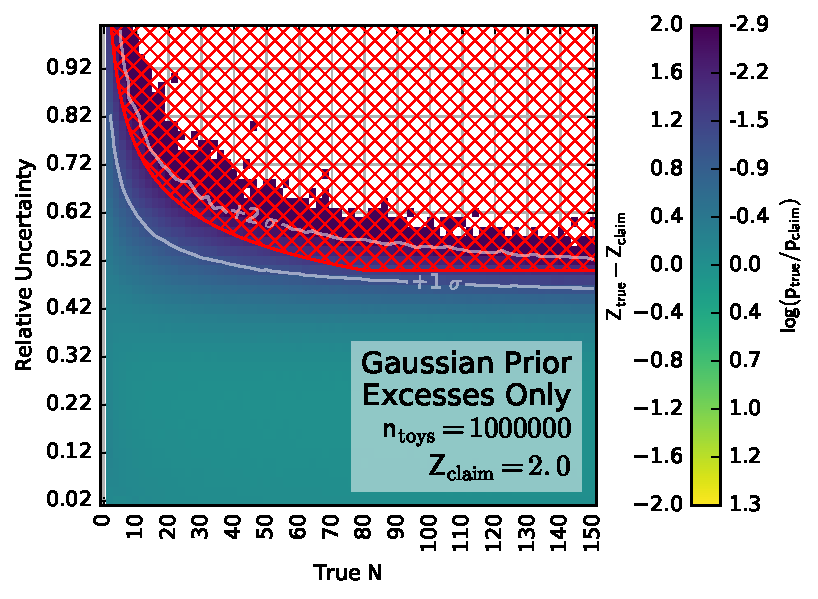
\includegraphics[width=\textwidth]{coverage/coverage_excess_normal_lin_thresh}
    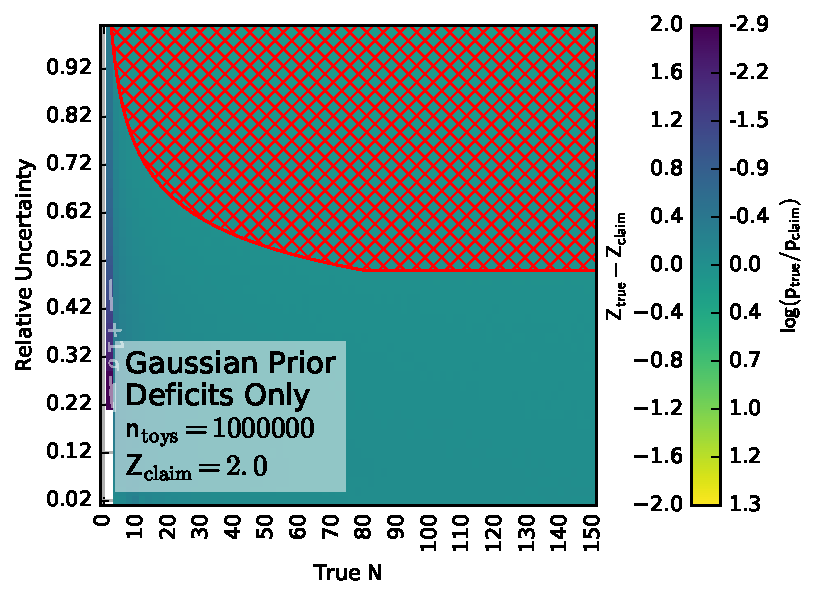
\includegraphics[width=\textwidth]{coverage/coverage_deficit_normal_lin_thresh}
    \caption{Illustration of the regions vetoed due to insufficient coverage (areas with red hatching pattern).}
    \label{fig:coverage_veto}
\end{figure}

\section{A Global $p$-Value}
\label{sec:global_pvalue}

\newcommand{\TSphat}{\ensuremath{T}\xspace}

The \ptilde distribution provides the ability to register less significant deviations in many classes by looking at the central part of the distribution. However, this manual method is only qualitative. We will now introduce a possible extension to the analysis which provides a quantitative method of combining the \ptilde values of all classes.

This not only allows us to draw conclusions about the presence of new physics in our observed data set, but also to quantify \ac{MUSiC}'s sensitivity for simulations of known benchmark models. Furthermore, an automated analysis can be used as regression test to decide whether future modifications to the analysis improve its sensitivity.

As before, the desired output for such a global method is a $p$-value which can then be compared to a significance threshold $\alpha$.
As input, the algorithm takes the look-elsewhere-corrected \ptilde values of all classes. In the case of \ac{MC} simulation, either for \ac{SM} or signal studies, such a set of \ptilde values can be provided for each pseudo experiment round, for observed data we only obtain one list (one value for each class).

The algorithm for the \ac{SM} distribution goes as follows: For each pseudo experiment round, the distribution of \ptilde values (of all classes) is compared to a reference distribution using a statistical test. The test outputs a scalar result \TSphat, where a larger value indicates a larger deviation from the reference distribution. \TSphat is then noted in a separate set, which eventually contains one test statistic value for each pseudo experiment round.
For observed data, the test statistic is calculated for the (only) set of \ptilde-values, resulting in $\TSphat_\text{data}$.

Finally, the resulting \phat value is defined as the rate of pseudo-rounds where $\TSphat > \TSphat_\text{data}$, similar to \ptilde before. This way, full coverage of \phat is guaranteed by definition.

For the quantification of sensitivity, the \emph{test power} $\beta$ for a given signal is calculated. The test power describes the probability that the \ac{SM} null hypothesis is (correctly) rejected if new physics are present in the data set. 
The \ac{SM}-step is applied as described above. \phat is then calculated for each signal pseudo experiment round, resulting in multiple $\TSphat_\text{signal}$ values. After agreeing on a significance threshold $\alpha$, $\beta$ is the rate of significant \TSphat values.

So far, the choice of statistical test and reference distribution is not specified. In the following, multiple options are discussed. The distribution of \ptilde values under investigation is denoted as $f(\ptilde)$, the reference distribution is $g(\ptilde)$. The cumulative distribution functions are $F(\ptilde)$ and $G(\ptilde)$ respectively. 

\begin{itemize}
    \item $\chi^2$-Test: This test is used to compare two binned distributions. For each bin $i'$, the difference between reference $g'_i$ and comparison $f_i$ is evaluated.
    \begin{equation}
        \TSphat = \frac{\chi^2}{\text{ndof}} = \frac{1}{\text{number of bins}} \sum_i^{\text{bins}} \frac{\left(f'_i - g'_i\right)^2}{g'_i}
    \end{equation}
    A disadvantage of this method is that binning discards information. Additionally, the method works best for large number of event classes.
    
    \item Kolmogorov-Smirnov: This test does not require binning. It compares the cumulative distribution functions of reference and comparison. The maximal distance between $F$ and $G$ is \TSphat.
    \begin{equation}
        \TSphat = \sup_x \abs{F(x) - G(x)}
    \end{equation}
    A disadvantage of this test statistic is that it is most sensitive to deviations in the center of the distribution. Additionally, only the largest difference is used for the result, instead of accumulating the difference.
    
    \item Cramér-von-Mises: The Cramér-von-Mises test statistic consists of the integral over the quadratic difference between the reference and compared cumulative distribution functions:
    \begin{equation}
        \TSphat = n \int_{-\infty}^{\infty}\left(F(x) - G(x)\right)^2 w(x)\, \dd F(x)
    \end{equation}
    where $w(x) = 1$.
    
    \item Anderson-Darling: This test is similar to the Cramér-von-Mises method, but uses $w(x) = \left[G(x)(1 - G(x))\right]^{-1}$ instead, thus giving more weight to both tails of the distribution.
    For this test, there exists a discrete version for comparing with a uniform distribution\cite{Stephens:EDFstatisticsgoodness} and a discrete version for $k$ samples\cite{Scholz:KsampleAnderson}. Both are implemented and used in this analysis.
    
    \item Simple: \TSphat is the ratio of \ptilde values below a critical value, in this case \num{0.1}.
\end{itemize}

A thorough comparison of the afore-mentioned test statistics can be found in \cite{Stephens:EDFstatisticsgoodness}.

For each of the mentioned test statistics, two different reference distributions have been tested: a uniform distribution and the empirical distribution of all \ptilde-values of all pseudo experiment rounds in the \ac{SM} sample.
While the former choice has the advantage of being able to identify whether the \ac{SM} distribution agrees with our assumptions, in practice the latter gives better sensitivity because of the direct comparison with the \ac{SM}. It is up to interpretation which approach is more correct.

The global method has been validated on a \ac{SM}-only sample. The \ac{SM}-only sample was used as signal input and a separate automated search, \ptilde and \phat calculation was performed. 
The resulting test power is $\beta \approx \alpha$, which agrees well with the expectation.


%
%
%necessity of a global p-value: quantification of deviation of p-tilde distribution
%quantification of test power towards known new physics models
%regression testing of features
%input: look-elsewhere corrected p-values for all classes and N rounds (SM, signal), or look-elsewhere corrected-pvalues for all classes and 1 round (data)
%output for data: p-value for this specific test and SM-scenario
%output for signal: distribution of p-values (?)
%
%suggested procedure:
%gather p-tilde-values for all classes and one round
%apply statistical test (KS, KS-referenced, AD, Chi2, Simple)
%apply definition of p-value: count "more extreme" outcomes
%problems: uniform reference vs SM-reference, binning (chi2), possibility of infinite p=1 classes (solution: low-stats treatment + cut at p<0.95)
%
%tests:
%KS: common nonparametric methods for comparing samples, unbinned, formula, disadvantage: more sensitive near center of distribution, max() instead of integration
%
%KS-referenced: as KS
%
%AD: quadratic EDF (empirical distribution function) test, integrates instead of max, weight in tails 
%
%Likelihood
%
%Simple test: count classes with p-tilde<0.1
%
%also tested: CvM (=AD with w=1)
%
%
%validation on SM: power approx alpha

% !TeX spellcheck = en_US
% !TeX encoding = UTF-8
% !TeX root = ../document.tex

\newcommand{\lumiA}{\SI{2.3}{\per\femto\barn}}
\newcommand{\lumiB}{\SI{35.9}{\per\femto\barn}}

\chapter{Discovery Potential}
\label{chap:sensitivity_studies}

The study of the discovery potential, also called \emph{sensitivity study}, has multiple purposes: On one hand, its goal is to assess the absolute sensitivity of the analysis towards certain benchmark models for new physics. But on the other hand, it can also be used to evaluate the sensitivity for a single model using different analysis variants. This allows us to assess which features, such as algorithms or parameters, have the largest impact on the discovery potential.

The chapter will start with the latter goal: After defining a set of features and key questions to be answered in this chapter, we will present the corresponding results in form of tables and graphics and move to a conclusion. 
In the second part, the sensitivity towards the benchmark models introduced earlier will be explicitly assessed and compared to dedicated analyses performed on a similar dataset by \ac{CMS}.

\subsubsection{Key Questions}
\begin{itemize}
    \item Validation: Using only the \ac{SM} as new physics input, are the \ptilde-distribution and \phat results inconclusive, as expected?
    \item How does the \ptilde distribution of the \ac{SM}-only scan scale with luminosity?
    \item How does the minimum-yield-per-event-class threshold (\fref{sec:min_yield}) affect the \ac{SM}-only distribution?
    \item How do the region vetoes (including the overcoverage veto introduced in \fref{sec:overcoverage_veto}) impact the available search space?
    \item Is \ac{MUSiC} sensitive to new physics that are only visible in one or few final states?
    \item Is \ac{MUSiC} sensitive to new physics that have a smaller impact on several final states?    
    \item Which test statistic for \phat shows the best sensitivity?
    %\item How does an increase in luminosity affect the sensitivity? For which kind of models does the analysis benefit from a higher luminosity?
    %\item How do \Pqb-tagged jets affect the sensitivity?
\end{itemize}

\subsection{Interpretation of the Result Plots}
\label{sec:how_to_read_plots}

The result figures presented in the following sections contain a large amount of information for readers not accustomed to \ac{MUSiC}. Therefore, this section aims to quickly introduce the material used to present the results and explain how they can be interpreted. An overview of the information presented is schematically shown in \fref{fig:results_flow}.

\begin{figure}
    \centering
    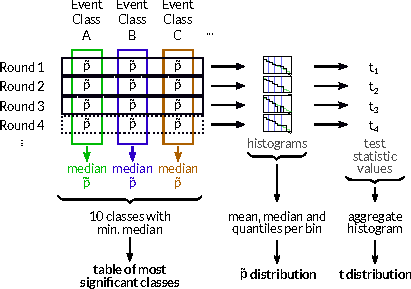
\includegraphics[width=0.7\textwidth]{ptilde_distrib_and_sign_classes}
    \caption{Flow of information from the sets of \ptilde values to the results presented in this chapter. The schematic shows the vertical aggregation of \ptilde values from $\nrounds = 4$ pseudo-experiments into median \ptilde values as well as the horizontal aggregation of distributions of \ptilde values for each round. Furthermore, the test statistic \TSphat is also computed horizontally and aggregated into a distribution.}
    \label{fig:results_flow}
\end{figure}

\subsubsection{\ptilde-Distribution}
This illustration has conceptually been introduced in \fref{sec:ptilde_distribution}. One example can be seen in \fref{fig:result_validation_ptilde}.
It is produced by aggregating $-\log_{10}{\ptilde}$ values: First, for each of the \nrounds rounds, the \nclasses results from \nclasses classes are sorted into a histogram. This results in \nrounds histograms, therefore \nrounds entries per bin. In each bin, the median bin content, the mean bin content and \SI{68}{\percent}- and \SI{95}{\percent} quantiles around the median are calculated. The highest bin serves as overflow bin, as we cannot obtain a precise value for $\ptilde < \num{1e-4}$ from \num{10000} \ac{SM}-only pseudo-experiments.

The aggregation procedure is done for the (corrected) \ptilde values originating from searches for deviations between the \ac{SM} and pseudo-experiments based on the \ac{SM} and its result is depicted in the turquoise and blue bands, as well as the turquoise line and the black dotted line. 
Additionally, the illustrations show a dashed green line which represents a uniform distribution. Because of the logarithmic binning, the number of uniform events is not equal for each bin. The uniform distribution can be used to tell whether \ptilde fulfills the requirement of a $p$-value of being uniformly distributed.

Results of the pseudo-experiments originating from a signal study (see \fref{sec:signal_study}) are depicted within the same figure as red data points. The vertical error bar around these points indicate the \SI{68}{\percent} quantiles around the median. This thesis uses \num{100} signal pseudo-experiments for each event class, thus \num{100} bin contents have been used to calculate the magnitude of the error bar.

\subsubsection{Table of Most Significant Classes}
The second result presentation is the table of most significant classes. It is aggregated by regarding the corrected \ptilde-values of each event class for all rounds. For each event class, the median \ptilde value is computed. Subsequently, the event classes with the \num{10} smallest medians are presented, alongside with the $Z$-score expressing the deviation in terms of standard deviations of a normal distribution (for the conversion formula, see \fref{app:z_score}). 

\subsubsection{Distributions of \TSphat}
The third way of presenting the results is by aggregating distributions of \TSphat values. Several examples are shown in \fref{fig:result_validation_phat}. There are always multiple distributions depicted in one figure: The distribution filled in gray shows the distribution of \TSphat values from \ac{SM}-pseudo-experiments. In addition there is at least one distribution from a signal study, drawn as a colored line. 

A vertical line indicates the critical value \TSphatcrit. It is defined as value of \TSphat separating $\alpha = \SI{5}{\percent}$ of the area under the \ac{SM}-only curve. The test power can also be read from the result figure as the area to the right of \TSphatcrit under each signal line.

\subsection{Validation Using the \ac{SM}}
The automated search takes two inputs when performing a sensitivity study: A set of event classes from classified events of the \ac{SM} only, and a set of event classes where simulated new physics events have been added to the \ac{SM} expectation. In order to validate the analysis, the latter input can be replaced by the same sample of \ac{SM}-only event classes. 

In this case, it is expected not to find a significant event class, there should be no significant deviation in the distribution of \ptilde values between the median signal rounds and the mean \ac{SM}-pseudo rounds, and the test power of the \phat test should be $1 - \beta \approx \alpha = \SI{5}{\percent}$.

The qualitative results of this validation run are depicted in \fref{fig:result_validation_ptilde}. As expected, the distribution of \ptilde values shows no deviation between the median bin contents for the signal study, indicated by the red data points and the median bin content of the \ac{SM}-only pseudo-experiments. The table below shows the \num{10} most significant event classes. The most significant class deviates by $\num{0.3}\sigma$, thus being in complete agreement with the expectation. 

\Fref{fig:result_validation_phat} shows results of the newly introduced global $p$-value. As expected, the gray \ac{SM}-only distribution and the blue validation distribution overlap for all test statistics. Furthermore, the expected test power is $1 - \beta = \alpha \approx \SI{5}{\percent}$, which confirms that we would find a significant deviation in the validation data set as often as in the \ac{SM}.

\begin{figure}
    \centering
    \includegraphics[width=\textwidth]{results/ptildeplots/signal,validation,bJets,SumPt/SM,bJets,SumPt/exclusive/pdf/p-tildeSumPt}
    {
        \begin{longtable}{l S[table-figures-integer=1,table-figures-decimal=2,table-comparator=true,table-figures-exponent=1] S[table-figures-integer=1,table-figures-decimal=1,table-comparator=true,table-figures-exponent=0]}
\toprule
{Event Class} & {Median \ptilde} & {$Z$} \\
\midrule
\endhead
\num{1} \Pe + \num{1} \Pmu + \MET + X & 2.00e-04 & 3.5 \\
\num{1} \Pe + \num{1} \Pmu + X & 5.00e-04 & 3.3 \\
\num{1} \Pe + X & 1.82e-02 & 2.1 \\
\num{1} \Pe + \num{1} \Pmu + \num{1} jet + \MET + X & 4.39e-02 & 1.7 \\
\num{1} \Pe + \num{1} \Pmu + \num{1} jet + X & 1.47e-01 & 1.1 \\
\num{1} \Pe + \MET + X & 1.50e-01 & 1.0 \\
\num{1} \Pe + \num{1} \Pmu + \num{2} jets + \MET + X & 3.48e-01 & 0.4 \\
\num{1} \Pe + \num{1} \Pphoton + X & 3.74e-01 & 0.3 \\
\num{2} \Pe + \num{1} \Pmu + \num{1} \Pphoton + \MET + X & 3.74e-01 & 0.3 \\
\num{1} \Pe + \num{1} \Pphoton + \num{3} jets + \MET + \num{2} b-jets + X & 3.93e-01 & 0.3 \\
\bottomrule
\end{longtable}
    }
    \caption{Distribution of \ptilde values and table of most significant classes for the \ac{SM}-only validation. For a detailed explanation on the information, see \fref{sec:how_to_read_plots}. As expected, no deviation between the validation (red data points) and the \ac{SM}-only pseudo-experiments (dotted line) is observed. 
    The table below shows the event classes with the smallest median of \ptilde between the signal simulation rounds. The most significant class shows a deviation of $\num{0.3}\sigma$, which is not significant.}
    \label{fig:result_validation_ptilde}
\end{figure}

\begin{figure}
    \centering
    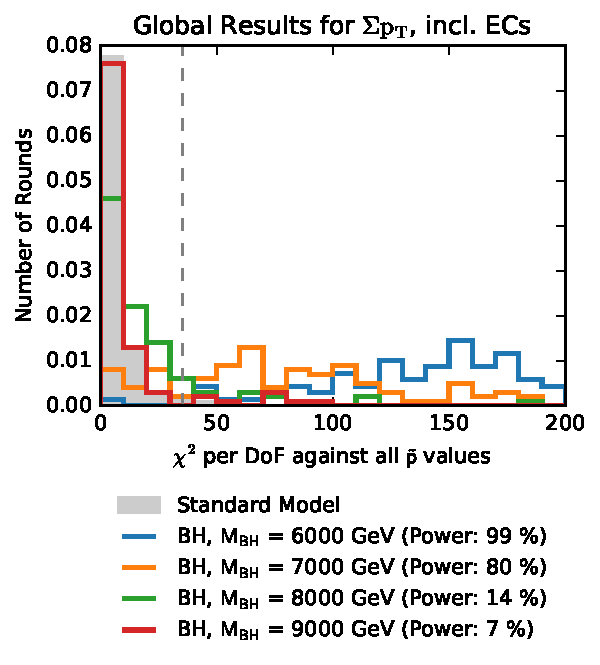
\includegraphics[height=7.5cm]{results/phatplots/bJets/VALIDATION/exclusive/SumPt/ChiSq_referenced_results}
    \includegraphics[height=7.5cm]{results/phatplots/bJets/VALIDATION/exclusive/SumPt/KS_referenced_results}
    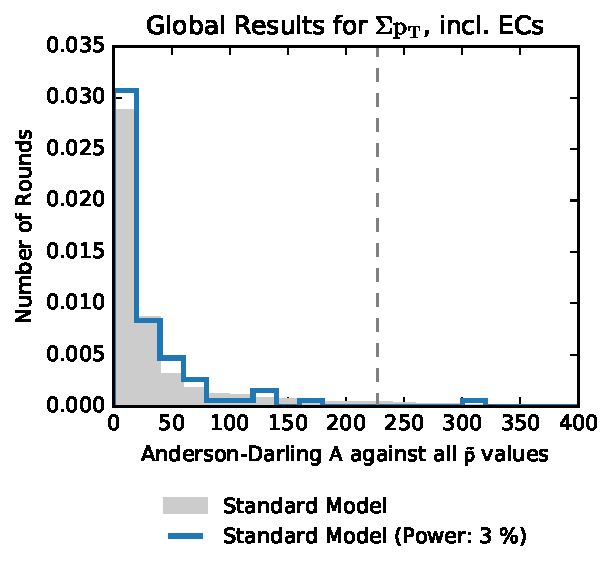
\includegraphics[height=7.5cm]{results/phatplots/bJets/VALIDATION/exclusive/SumPt/AD_referenced_results}
    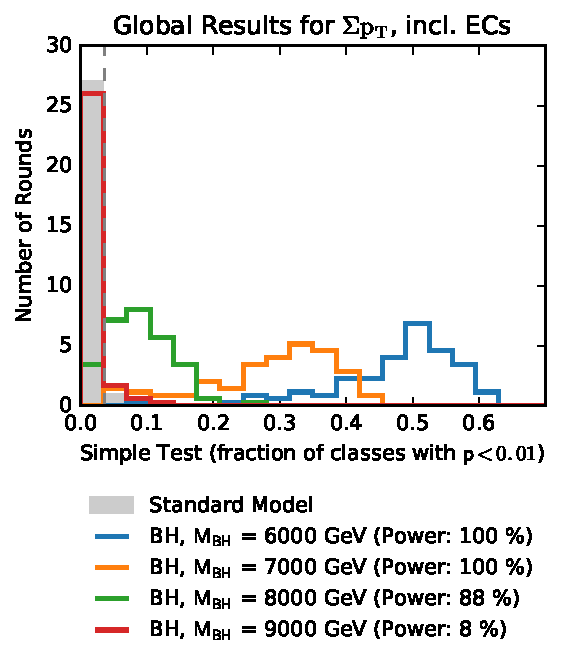
\includegraphics[height=7.5cm]{results/phatplots/bJets/VALIDATION/exclusive/SumPt/Simple_results}
    \caption{Distribution of \TSphat values of the validation run. As expected, the test power of the null-hypothesis is about \SI{5}{\percent} and no significant deviation between the two distributions is apparent.}
    \label{fig:result_validation_phat}
\end{figure}

\subsection{Differences between Luminosity of \lumiA and \lumiB}
To assess the differences between the luminosities of the data taking periods in 2015 (with a luminosity of \lumiA) and 2016 (\lumiB), we can compare the results from the \ptilde distribution in \fref{fig:result_validation_ptilde} to similarly obtained results in \fref{fig:result_lumi2016_ptilde}. For this distribution, all event yields have been scaled to the new luminosity and the automated search was repeated. Because of the increase in the scaled event yield, more event classes will pass the threshold of $\Nmc \geq \num{0.01}$, therefore more event classes will be searched for deviations in the 2016 dataset. This also shows e.g. in the number of exclusive event classes, which rises from \num{460} to \num{716}. 

\begin{figure}
    \centering
    \includegraphics[width=\textwidth]{results/ptildeplots16/signal,validation,bJets,SumPt/SM,bJets,SumPt/exclusive/pdf/p-tildeSumPt}
    \caption{Distribution of \ptilde values for the \ac{SM}-only validation using the \lumiB.}
    \label{fig:result_lumi2016_ptilde}
\end{figure}

The validation procedure presented in the previous chapter was also applied on the dataset with the luminosity of \lumiB, as depicted in red in \fref{fig:result_lumi2016_ptilde}. Again, no deviation between the validation dataset and the \ac{SM}-only pseudo-experiments is visible.

\subsection{Effect of the Minimum Yield Threshold}
The minimum yield threshold was introduced in \fref{sec:min_yield} in order to suppress the creation of almost-empty event classes, as the discretization of the \TS- and \ptilde-values would invalidate the interpretation of the \ptilde value as a probability. This effect has been analyzed by performing automated searches and aggregating distributions of \ptilde-values with several different values of the minimum yield threshold. The results are presented in \fref{fig:result_minyield_ptilde} and \fref{tab:result_minyield_table}. 

\begin{figure}
    \centering
    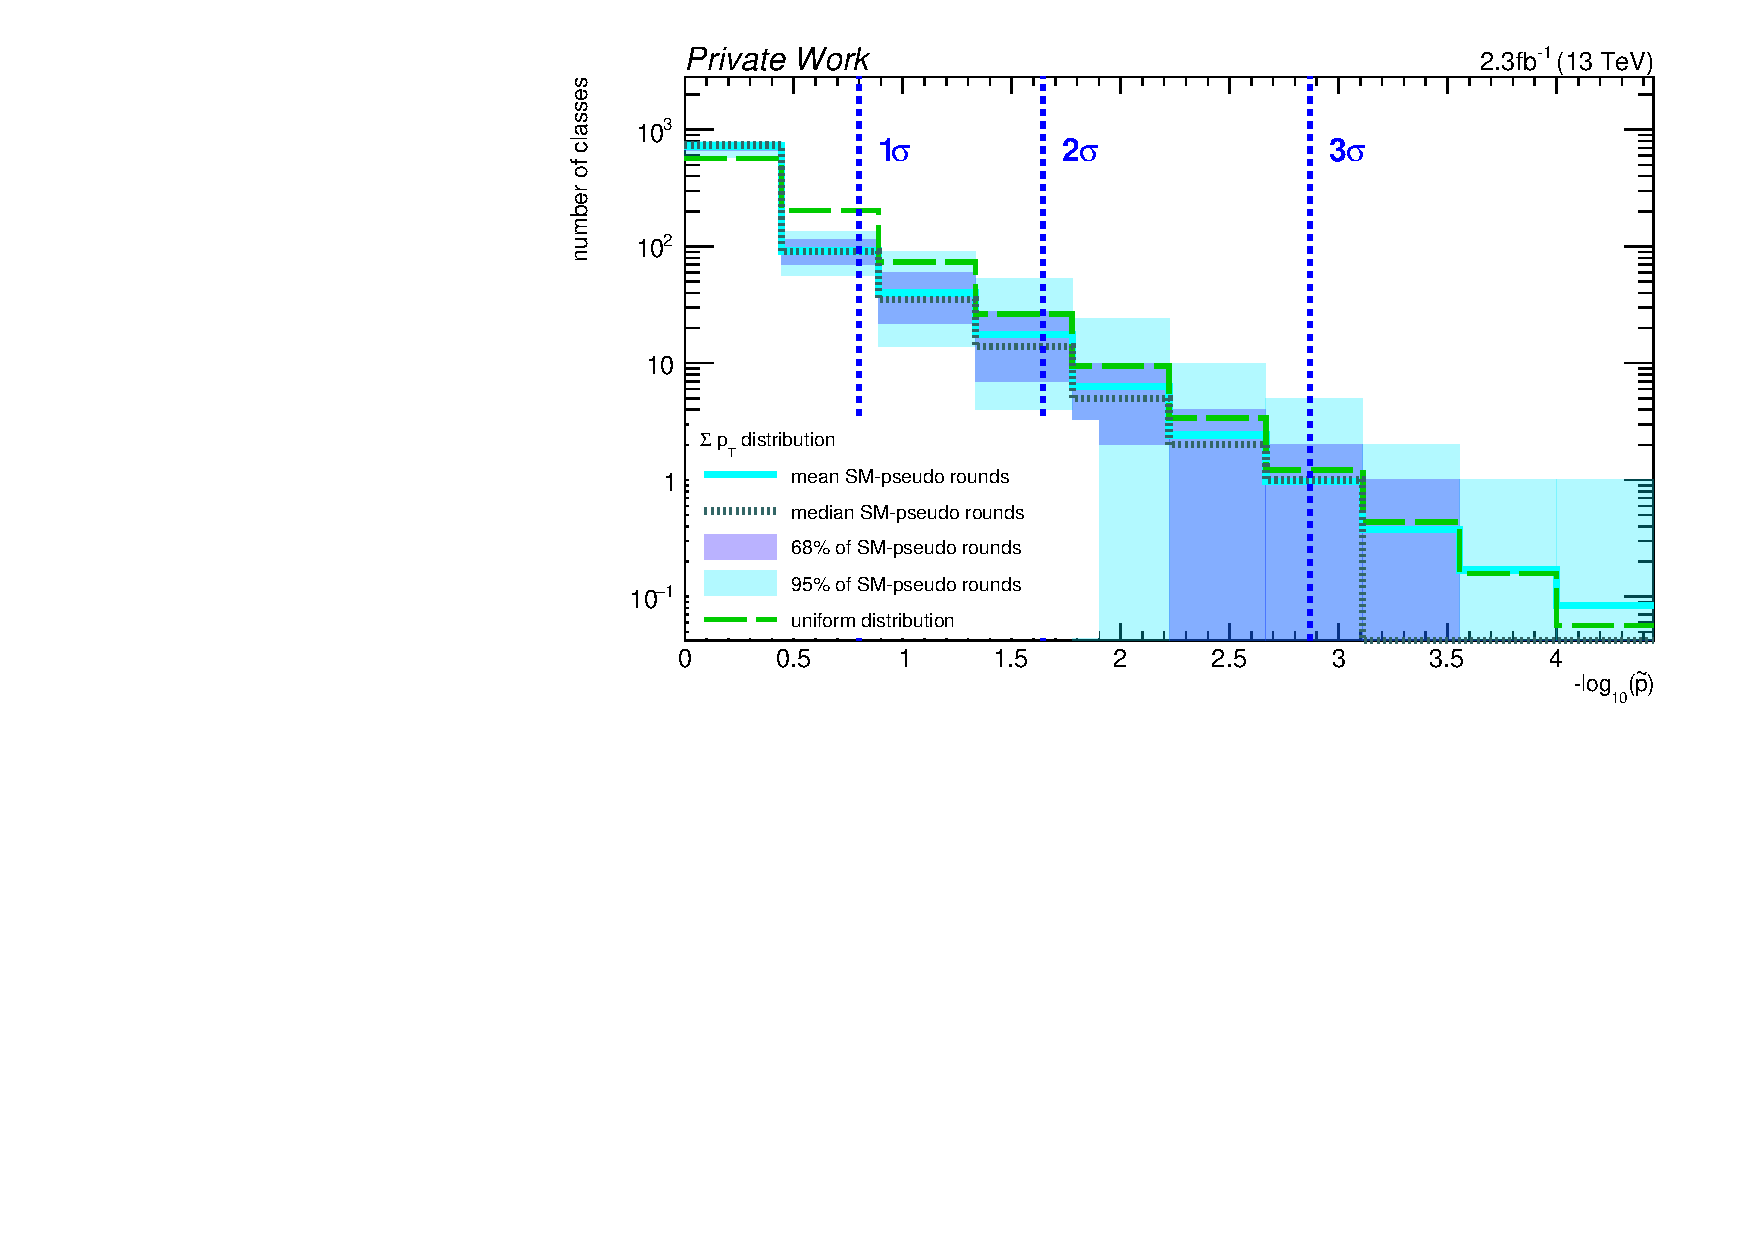
\includegraphics[width=\textwidth]{results/minyieldplots/no_minyield/plotOut/pdf/p-tildeSumPt}
    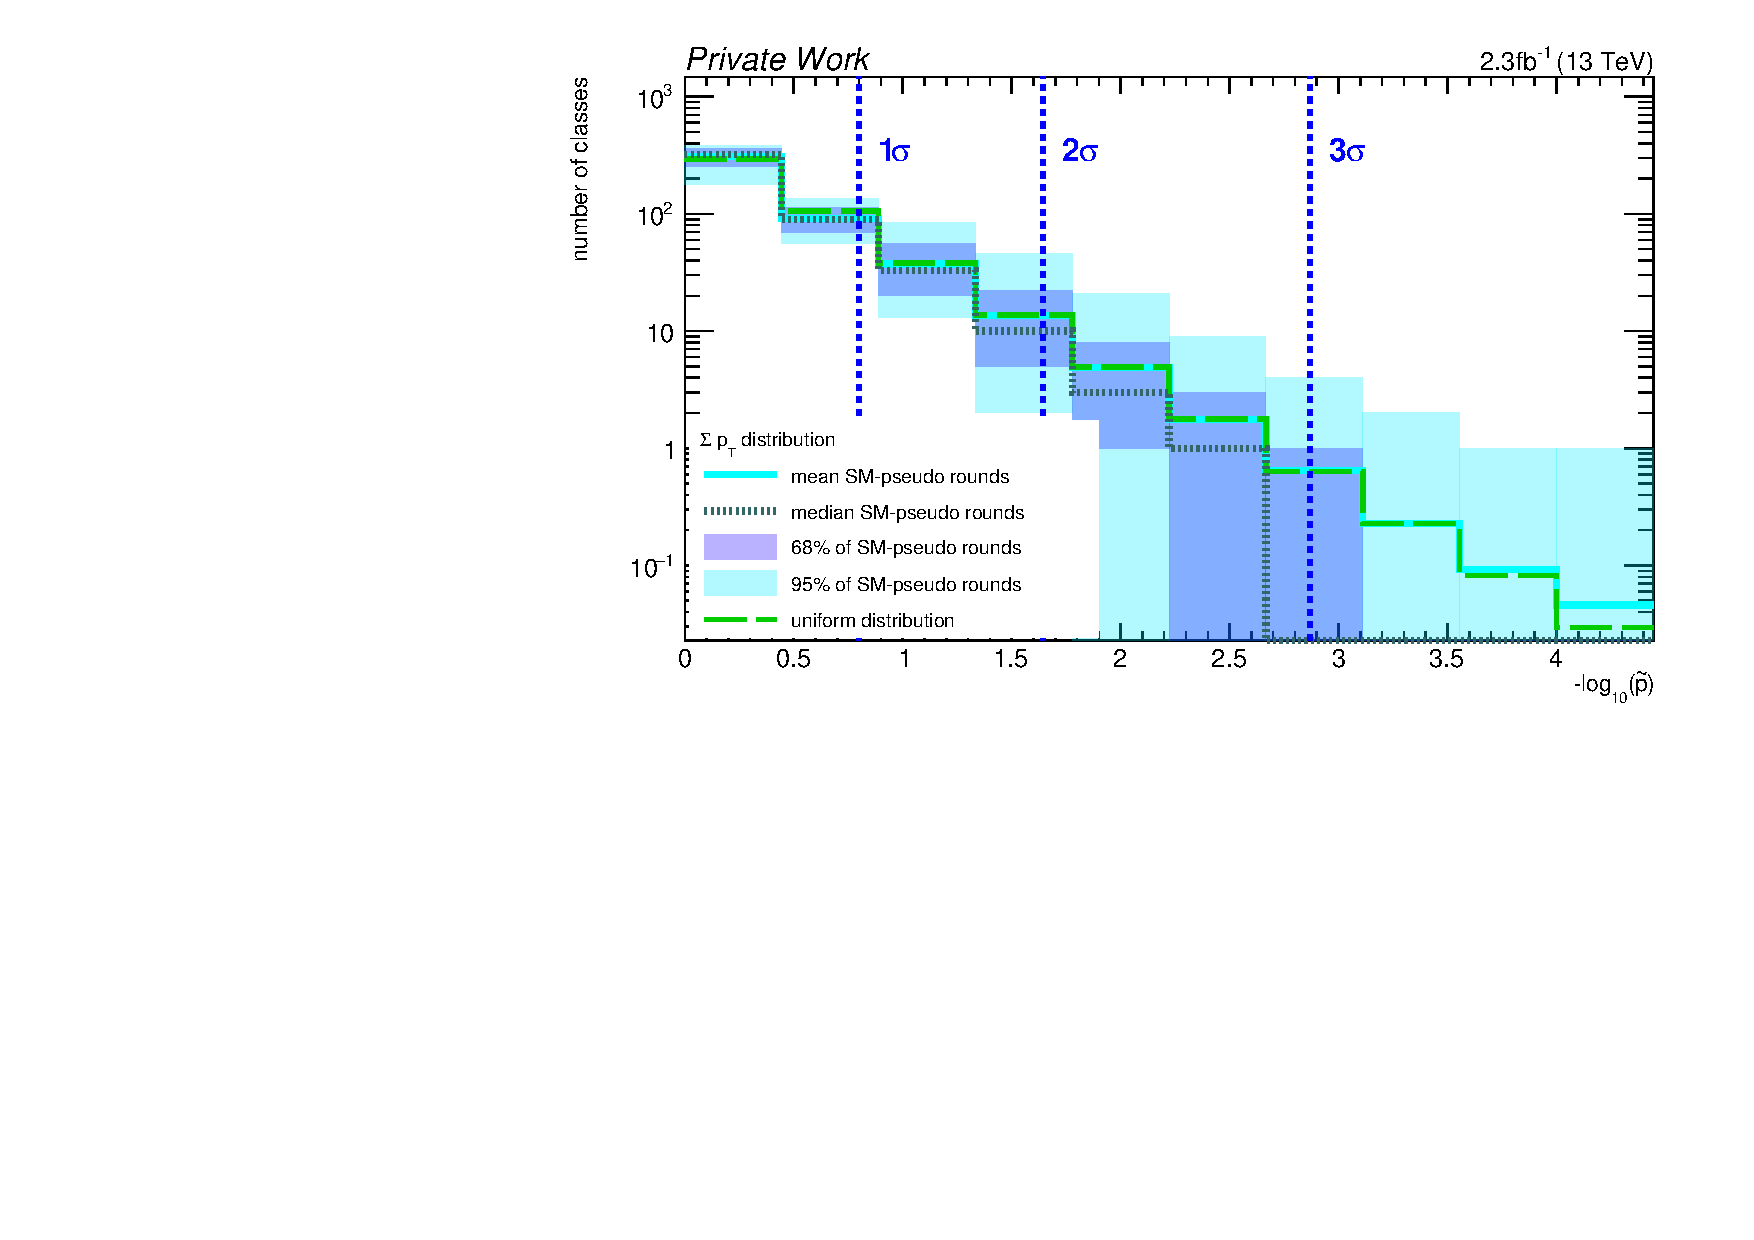
\includegraphics[width=\textwidth]{results/minyieldplots/minyield01/plotOut/pdf/p-tildeSumPt}
    \caption{Distribution of \ptilde values for different minimum yield thresholds at \lumiA. The distribution above was created with a threshold of \num{0}, the second one with a threshold of \num{0.1}. Although the standard model and its validation agree in the upper illustration, neither distribution is in accordance with a uniform distribution. Therefore, the validity of \ptilde without such a threshold is questionable.}
    \label{fig:result_minyield_ptilde}
\end{figure}

The first \ptilde distribution has been generated with $\Nmc \geq \num {0}$, only filtering out event classes with negative total event yield. The \ac{SM}-only distribution clearly shows deviations from the uniform distribution, especially in the bins containing less significant event classes. This is not the case in the second figure, showing a distribution generated with $\Nmc \geq \num{0.1}$, the threshold chosen for this thesis.

\begin{table}
    \centering
    Event classes created with a luminosity of \lumiA:
    \begin{tabular}{l S S S S S}
        \toprule
        & {without thresh.} & {$\Nmc \geq \num{0}$} & {$\Nmc \geq \num{0.01}$} & {$\Nmc \geq \num{0.1}$} & {$\Nmc \geq \num{1}$} \\
        \midrule
        exclusive     & 1249 & 1190 & 666 & 460 & 239 \\
        jet-inclusive & 1359 & 1291 & 738 & 508 & 343 \\
        inclusive     & 1686 & 1602 & 934 & 672 & 465 \\
        \bottomrule
    \end{tabular}
    \vspace{1em} \\
    Event classes created with a luminosity of \lumiB:
    \begin{tabular}{l S S S S S}
            \toprule
            & {without thresh.} & {$\Nmc \geq \num{0}$} & {$\Nmc \geq \num{0.01}$} & {$\Nmc \geq \num{0.1}$} & {$\Nmc \geq \num{1}$} \\
            \midrule
            exclusive     & 1249 & 1190 & 888 & 716 & 492 \\
            jet-inclusive & 1359 & 1291 & 936 & 787 & 547 \\
            inclusive     & 1686 & 1602 & 1246 & 996 & 709 \\
            \bottomrule
        \end{tabular}
    \caption{Number of event classes created with several minimum yield threshold at a luminosity of \lumiA (upper table) and \lumiB (lower table).}
    \label{tab:result_minyield_table}
\end{table}

In addition, one can regard the reduction in the number of event classes between several threshold values, as shown in \fref{tab:result_minyield_table}. Overall, the minimum yield threshold reduces the number of event classes by more than a factor of two for the 2015 dataset. Because the same \ac{MC} simulated events were used for the 2015 and 2016 scenarios, the number of initial event classes remains the same between the studies. The increase in luminosity by a factor of \num{16} however causes more event classes to pass the threshold. Therefore the latter dataset is less affected by the threshold.

\subsection{Impact of Vetos}
In \fref{sec:region_veto}, several rules have been introduced that aim to exclude regions from the automated search where the \ac{SM} simulation is incomplete and therefore no inference can be made. The set of rules was expanded in \fref{sec:overcoverage_veto} in order to avoid statistical inference on regions where our test statistic is known to be incorrect because of overcoverage.

In this section, we would like to assess the impact of the region vetoes on the number of regions that are searched for deviations. 
The numbers in \fref{tab:result_veto} have been obtained by recording the reason for each veto during an automated search on the \sumpT distribution of \ac{SM}-only pseudo-experiments. Because the vetoes are evaluated in a given order, aborting after the first matching rule, the numbers on the latter vetoes are only an approximation and a lower bound. The total number of vetoes, however, can be accurately determined using this feature.

\begin{table}
    \centering
    \begin{tabular}{l r r}
        \toprule
        {veto reason} & {vetoed regions} & {percentage of $x$-axis}\\
        \midrule
        empty bin added & \SI{38.8}{\percent} & \SI{35.6}{\percent} \\
        \textbf{overcoverage threshold (\fref{sec:overcoverage_veto})} & \SI{4.9}{\percent} & \SI{5.6}{\percent} \\
        negative total yield & \SI{1.0}{\percent} & \SI{0.5}{\percent} \\
        large negative contribution of any process & \SI{2.5}{\percent} & \SI{2.0}{\percent} \\
        negative/low leading contribution & \SI{5.3}{\percent} & \SI{4.4}{\percent} \\
        large statistical uncertainty & \SI{6.2}{\percent} & \SI{4.3}{\percent} \\
        \midrule
        total vetoed & \SI{58.7}{\percent} & \SI{52.4}{\percent} \\
        \bottomrule
    \end{tabular}
    \caption{Impact of region vetoes. The vetoes are applied in the order listed here. The percentage noted in the second column indicates the number of regions removed in each step. The first reason "empty bin added", which is not explained in \fref{sec:region_veto}, originates from an optimization where the test statistic \TS is not recomputed after an empty bin has been added to the region.}
    \label{tab:result_veto}
\end{table}

In addition to the aforementioned rules, the entry "empty bin added" is listed. This is due to an optimization in the automated search, where regions are not reassessed after an empty bin has been added. The motivation behind this optimization is that the value of \TS would be the same (as neither \Nmc, \sigmamc or \Ndata change) and the region would be larger, therefore not a candidate to become \ac{RoI}.

Overall, more than half of the regions (\SI{58.7}{\percent}) are skipped. However, the optimization accounts for \SI{38.8}{\percent}, leaving only about \SI{20}{\percent} to the rules that prevent an invalid inference. The newly introduced veto amounts for about \SI{5}{\percent} of vetoed regions.


\subsection{Comparison of Test Statistics}
In this section, the results of using several test statistics on the semiclassical black hole model are explored. The distributions of the four aforementioned test statistics can be found in \fref{fig:results_test_statistics}. The test power towards each model is indicated in the legend and in this case varies between \SI{53}{\percent} and \SI{82}{\percent} for the given test statistics.

\begin{figure}
    \centering    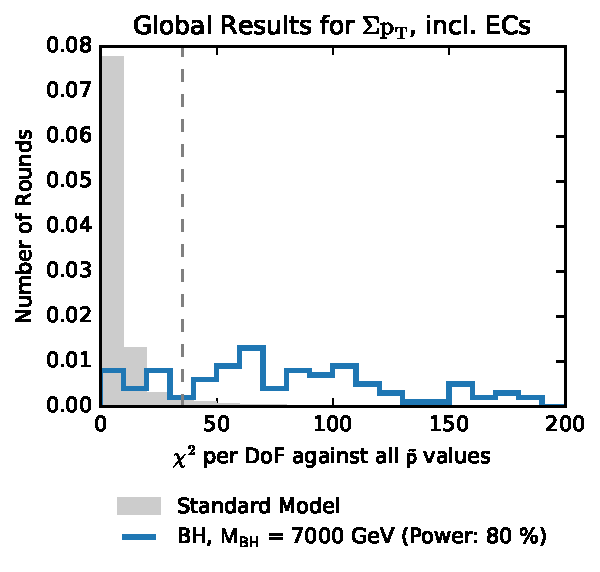
\includegraphics[height=7cm]{results/phatplots/bJets/BH_DEMO/inclusive/SumPt/ChiSq_referenced_results}
    \includegraphics[height=7cm]{results/phatplots/bJets/BH_DEMO/inclusive/SumPt/KS_referenced_results}
    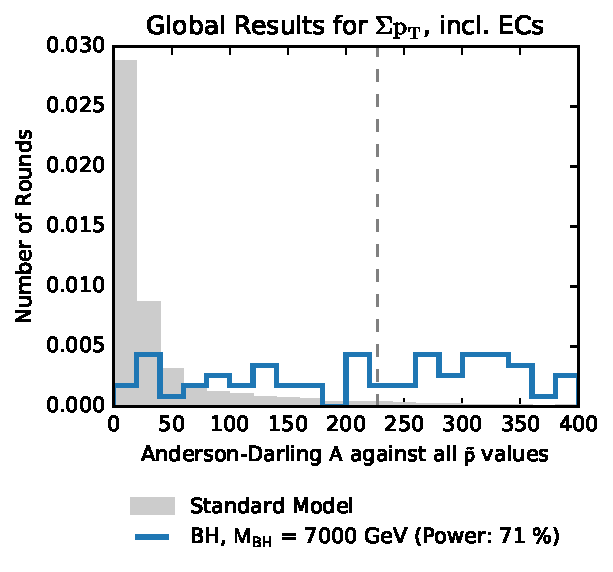
\includegraphics[height=7cm]{results/phatplots/bJets/BH_DEMO/inclusive/SumPt/AD_referenced_results}
    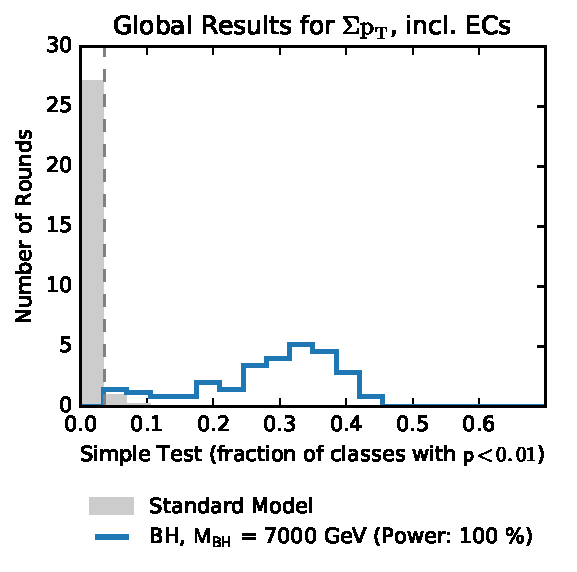
\includegraphics[height=7cm]{results/phatplots/bJets/BH_DEMO/inclusive/SumPt/Simple_results}
    \caption{Comparison of test statistics for the \ac{BH} model. For demonstration purposes, the test statistic values of the semiclassical black hole at $M_\text{BH} = \SI{7000}{\GeV}$ signal study are drawn. The deviations between the two distributions in each figure are clearly visible. In this case, the simple test shows the largest power (\SI{83}{\percent}), followed by the $\chi^2$ test. In any case, the median value for \TSphat is beyond \TSphatcrit.}
    \label{fig:results_test_statistics}
\end{figure}

The largest test power is given by the "simple" test statistic. While this may appear surprising at first, considering that the other test statistics are much more sophisticated, there exists a possible explanation: In the past, the \ac{MUSiC} analysis has been developed while assessing the sensitivity by eye from the \ptilde-distribution. The \ptilde-distribution, which is binned in logarithmic bin sizes, strongly favors deviations in bins with $\ptilde \rightarrow 0$. Therefore, the analysis might have been optimized for this area of sensitivity.
Only now, with the introduction of a quantitative measure for deviations in the bulk of the distribution, we can start to also optimize for sensitivity in this region. Therefore, the test power of these statistical test should be considered alongside the "simple" test during future design decisions of the analysis.

\subsection{Sensitivity in Few Final States}
The \ac{QBH} model serves as benchmark for new physics that appear in few final states. Since the simulated black holes are assumed to decay completely into a \Pe + \Pmu pair, this final state is expected to dominate the list of significant classes.

To illustrate this, we regard the \ac{QBH} dataset with the $M = \SI{4000}{\GeV}$ black hole mass. It is the highest mass point for this model that generates a significant excess. The results of the analysis are presented as a distribution of \ptilde values and table of most significant classes in \fref{fig:results_few_final_states}.

\begin{figure}
    \centering
    \includegraphics[width=\textwidth]{results/ptildeplots/signal,QBH_M-4000,bJets,SumPt/SM,bJets,SumPt/jet-inclusive/pdf/p-tildeSumPt}
    {
        \begin{longtable}{l S[table-figures-integer=1,table-figures-decimal=2,table-comparator=true,table-figures-exponent=1] S[table-figures-integer=1,table-figures-decimal=1,table-comparator=true,table-figures-exponent=0]}
\toprule
{Event Class} & {Median \ptilde} & {$Z$} \\
\midrule
\endhead
\num{1} \Pe + \num{1} \Pmu + \MET + X & 2.00e-04 & 3.5 \\
\num{1} \Pe + \num{1} \Pmu + X & 5.00e-04 & 3.3 \\
\num{1} \Pe + X & 1.82e-02 & 2.1 \\
\num{1} \Pe + \num{1} \Pmu + \num{1} jet + \MET + X & 4.39e-02 & 1.7 \\
\num{1} \Pe + \num{1} \Pmu + \num{1} jet + X & 1.47e-01 & 1.1 \\
\num{1} \Pe + \MET + X & 1.50e-01 & 1.0 \\
\num{1} \Pe + \num{1} \Pmu + \num{2} jets + \MET + X & 3.48e-01 & 0.4 \\
\num{1} \Pe + \num{1} \Pphoton + X & 3.74e-01 & 0.3 \\
\num{2} \Pe + \num{1} \Pmu + \num{1} \Pphoton + \MET + X & 3.74e-01 & 0.3 \\
\num{1} \Pe + \num{1} \Pphoton + \num{3} jets + \MET + \num{2} b-jets + X & 3.93e-01 & 0.3 \\
\bottomrule
\end{longtable}
    }
    \caption{Distribution of \ptilde values and most significant exclusive event classes for the quantum black hole decaying to $\Pe + \Pmu$, $M = \SI{4000}{\GeV}$.}
    \label{fig:results_few_final_states}
\end{figure}

As expected, the set of most significant classes is dominated by final states containing an \Pe and \Pmu pair. The most significant event class \eventclass{1\Pe + 1\Pmu + \MET jet incl.} has $\ptilde < \num{1e-4}$. This inequality indicates that in none of the \num{10000} \ac{SM}-only pseudo-experiments, a more significant deviation has been found. 
More detailed information can be gained by looking at the kinematic distribution directly. For this reason, it is explicitly shown in \fref{fig:qbh_most_significant_class}.
Due to lepton flavor conservation, the \Pe + \Pmu pair cannot be created from the decay of a single \ac{SM} particle. However, the decay of a \Ptop + \APtop pair can directly affect this final state if both \PW bosons decay into leptons. Additionally, this process gives rise to a significant amount of \MET as well as two additional jets. 
For these reasons, the \Ptop + \APtop decay dominates the most significant event class by contributing approximately \num{720} of \num{850} events. However, the spectrum falls steeply and the \ac{SM} contribution is negligible for $\sumpT \gtrapprox \SI{1500}{\GeV}$. In this region, the \ac{QBH} signal dominates, although the total contribution is \num{2.4} events.

\begin{figure}
    \centering
    \includegraphics[width=\textwidth]{results/ec_plots/QBH_M-4000_n4/plotOut/pdf/EventClass/SumPt/Rec_1Ele_1Muon_1MET+NJetsSumPt}
    \includegraphics[width=\textwidth]{results/ec_plots/QBH_M-4000_n4/plotOut/pdf/EventClass/SumPt/Rec_1Ele_1Muon+NJetsSumPt}
    \caption{Classification output for the two most significant classes of the black hole model at $M = \SI{4000}{\GeV}$, distribution of \sumpT kinematic variable: \eventclass{1\Pe + 1\Pmu + \MET jet incl.} and \eventclass{1\Pe + 1\Pmu jet incl.}.}
    \label{fig:qbh_most_significant_class}
\end{figure}

The second most significant event class is the expected final state \eventclass{1\Pe + 1\Pmu jet incl.}. The amount of signal events in this class is comparable to the \eventclass{1\Pe + 1\Pmu + \MET jet incl.} class (\SI{2.6} events). However, as more \ac{SM} process can contribute directly, the \ac{SM} yield in this class is about \num{3400} events. Its significance in the signal study is $\num{1.1}\sigma$. 
The third most significant event class is completely insignificant with a $Z$-score of $\num{0.9}\sigma$.

The \ptilde distribution indicates a similar result: There is no apparent deviation within the bulk of the distribution, but the overflow bin contains one event class in the median, occasionally also none or two event classes. However, overall the distribution is compatible with the prediction from \ac{SM}-only pseudo-experiments, showing that the distribution of \ptilde values alone does not suffice for discovering new physics as represented by this part of the analysis.

\subsection{Sensitivity in Multiple Final States}
As opposed to the previous section, the goal of this section is to assess sensitivity of the \ac{MUSiC} analysis towards new physics that appear as insignificant deviations in multiple final states. The benchmark model for this analysis is the semiclassical \acl{BH} model at the $M_\text{BH} = \SI{8000}{\GeV}$.
Similarly to the previous section, the results are first presented as distribution of \ptilde values and as a table of most significant classes in \fref{fig:multiple_final_states}.

\begin{figure}
    \centering
    \includegraphics[width=\textwidth]{results/ptildeplots/signal,BlackHole_MBH-8000,bJets,SumPt/SM,bJets,SumPt/jet-inclusive/pdf/p-tildeSumPt}
    {
        \begin{longtable}{l S[table-figures-integer=1,table-figures-decimal=2,table-comparator=true,table-figures-exponent=1] S[table-figures-integer=1,table-figures-decimal=1,table-comparator=true,table-figures-exponent=0]}
\toprule
{Event Class} & {Median \ptilde} & {$Z$} \\
\midrule
\endhead
\num{1} \Pe + \num{1} \Pmu + \MET + X & 2.00e-04 & 3.5 \\
\num{1} \Pe + \num{1} \Pmu + X & 5.00e-04 & 3.3 \\
\num{1} \Pe + X & 1.82e-02 & 2.1 \\
\num{1} \Pe + \num{1} \Pmu + \num{1} jet + \MET + X & 4.39e-02 & 1.7 \\
\num{1} \Pe + \num{1} \Pmu + \num{1} jet + X & 1.47e-01 & 1.1 \\
\num{1} \Pe + \MET + X & 1.50e-01 & 1.0 \\
\num{1} \Pe + \num{1} \Pmu + \num{2} jets + \MET + X & 3.48e-01 & 0.4 \\
\num{1} \Pe + \num{1} \Pphoton + X & 3.74e-01 & 0.3 \\
\num{2} \Pe + \num{1} \Pmu + \num{1} \Pphoton + \MET + X & 3.74e-01 & 0.3 \\
\num{1} \Pe + \num{1} \Pphoton + \num{3} jets + \MET + \num{2} b-jets + X & 3.93e-01 & 0.3 \\
\bottomrule
\end{longtable}
    }
    \caption{Distribution of \ptilde values and most significant exclusive event classes for the black hole model at the mass of $M_\text{BH} = \SI{8000}{\GeV}$.}
    \label{fig:multiple_final_states}
\end{figure}

The table of most significant classes shows, in contrast to the previous case, that there is no single event class that stands out with a large significance. The most significant event class has a $Z$-score of $\num{2.4}\sigma$, followed by three more event classes just above $\num{2}\sigma$.

However, it is noticeable that every single one of the ten most significant classes contain exactly one lepton, any number of jets and \MET. As mentioned in the introductory chapter, the branching ratio of the semiclassical black hole is proportional to the number of degrees of freedom of the decay products. Thus, quarks and gluons, which carry additional degrees of freedom through color charge, are heavily favored, resulting in multiple jets in the final state. 
A significant amount of \MET is also expected to appear during the evaporation of the black hole\cite{CMS:CMS-PAS-EXO-15-007}.
The single lepton in all of the most significant classes is caused by the choice of trigger rules, which require at least one lepton in each event.

For this model, the distribution of \ptilde values is very sensitive. During each round, there were about six event classes with $\ptilde < \num{1e-4}$, making the deviation from the \ac{SM}-only distribution highly significant. Note that the event classes which are sorted into the last bin vary between pseudo-experiment round and therefore do not appear with the same significance in the results table.


\subsection{Dependence on the Luminosity}
In the previous section, the highest discoverable mass points of the \ac{QBH} and \ac{BH} models have been presented, with respect to a luminosity of \lumiA. In this section, we will revisit the results, this time with the luminosity scenario of 2016 (\lumiB). The corresponding distributions are depicted in \fref{fig:results_lumichange}. 

\begin{figure}
    \centering
    \includegraphics[width=\textwidth]{results/ptildeplots16/signal,QBH_M-4000,bJets,SumPt/SM,bJets,SumPt/jet-inclusive/pdf/p-tildeSumPt}
    \includegraphics[width=\textwidth]{results/ptildeplots16/signal,BlackHole_MBH-8000,bJets,SumPt/SM,bJets,SumPt/jet-inclusive/pdf/p-tildeSumPt}
    \caption{Distributions of \fref{fig:qbh_most_significant_class} and \fref{fig:multiple_final_states} for the 2016 scenario with a luminosity of \lumiB, using the same models and mass points. On top: \acl{QBH} model with $M = \SI{4000}{\GeV}$, below: \acl{BH} model with $M_\text{BH} = \SI{8000}{\GeV}$.}
    \label{fig:results_lumichange}
\end{figure}

The figure on top shows the result for the \ac{QBH} model with a black hole mass of $M = \SI{4000}{\GeV}$. At \lumiA, there was one class belonging to the overflow bin on average. One can see that this number has increased at \lumiB, showing six event classes in the same bin on average. The bulk of the distribution, however, remains unchanged: No significant deviations are apparent in all but the highest histogram bin.

The second figure shows the distribution of \ptilde models from pseudo-experiments based on the \ac{BH} model. This model highly benefits from the increase in luminosity. On average, there are \num{16} classes in the overflow bin. A possible reason is that more event classes pass the $\Nmc \geq \num{0.1}$ threshold, including event classes that become available solely through the new physics model. In \fref{sec:results}, we will see that the highest mass point discoverable with a luminosity of \lumiB is $M = \SI{9000}{\GeV}$.

%\subsection{Benefits from \Pqb-Tagged Jets}



\section{Results by Model}
\label{sec:results}

The following sections aim to present absolute sensitivity results towards the tested benchmark models. As the cross section of each model decreases with the mass of the new physics object (black hole, \PSigma or \PWprime), we will show the full result set consisting of a distribution of \ptilde values, the table of most significant classes as well as the distribution of \TSphat values, for the highest mass that the analysis would be able to discover. 

For this purpose, we claim that a model would be discoverable if any of the following conditions are met: The distribution of \ptilde values shows a considerable deviation, the most significant event class has a median $Z$-score of more than $\num{3}\sigma$ or the test power of \TSphat is larger than \SI{50}{\percent}, i.e. the median \TSphat is larger than \TSphatcrit.

\subsection{Semiclassical Black Hole}
\label{sec:results_bh}

The results for the semiclassical black hole theory have already been presented and discussed in the previous sections. At a luminosity of \lumiA, the largest black hole mass that the \ac{MUSiC} analysis is sensitive is about $M_\text{BH} = \SI{8000}{\GeV}$. In this case, the distribution of \ptilde values shows an excess in the overflow bin, although no single event class has a $Z$-score larger than $\num{3}\sigma$.

Increasing the luminosity from \lumiA to \lumiB additionally enables sensitivity up to a black hole mass of $M_\text{BH} = \SI{9000}{\GeV}$, as shown in \fref{fig:result_bh_9000}. However, the decision about sensitivity towards this model is inconclusive as the \ptilde-distribution only shows a moderate deviation. 
\begin{figure}
    \centering
    \includegraphics[width=\textwidth]{results/ptildeplots16/signal,BlackHole_MBH-9000,bJets,SumPt/SM,bJets,SumPt/jet-inclusive/pdf/p-tildeSumPt}
    {
        \begin{longtable}{l S[table-figures-integer=1,table-figures-decimal=2,table-comparator=true,table-figures-exponent=1] S[table-figures-integer=1,table-figures-decimal=1,table-comparator=true,table-figures-exponent=0]}
\toprule
{Event Class} & {Median \ptilde} & {$Z$} \\
\midrule
\endhead
\num{1} \Pe + \num{1} \Pmu + \MET + X & 2.00e-04 & 3.5 \\
\num{1} \Pe + \num{1} \Pmu + X & 5.00e-04 & 3.3 \\
\num{1} \Pe + X & 1.82e-02 & 2.1 \\
\num{1} \Pe + \num{1} \Pmu + \num{1} jet + \MET + X & 4.39e-02 & 1.7 \\
\num{1} \Pe + \num{1} \Pmu + \num{1} jet + X & 1.47e-01 & 1.1 \\
\num{1} \Pe + \MET + X & 1.50e-01 & 1.0 \\
\num{1} \Pe + \num{1} \Pmu + \num{2} jets + \MET + X & 3.48e-01 & 0.4 \\
\num{1} \Pe + \num{1} \Pphoton + X & 3.74e-01 & 0.3 \\
\num{2} \Pe + \num{1} \Pmu + \num{1} \Pphoton + \MET + X & 3.74e-01 & 0.3 \\
\num{1} \Pe + \num{1} \Pphoton + \num{3} jets + \MET + \num{2} b-jets + X & 3.93e-01 & 0.3 \\
\bottomrule
\end{longtable}
    }
    \caption{Distribution of \ptilde values and most significant exclusive event classes for the black hole model at the mass of $M_\text{BH} = \SI{9000}{\GeV}$.}
    \label{fig:result_bh_9000}
\end{figure}

\subsection{Quantum Black Hole}
\label{sec:results_qbh}

Similarly to the semiclassical black hole, the results regarding the \ac{QBH} model have also been presented earlier in this chapter. In \fref{fig:results_few_final_states}, sensitivity to the \ac{QBH} model up to a black hole mass of $M = \SI{4000}{\GeV}$ is demonstrated.

With an increased luminosity of \lumiB, the analysis becomes sensitive up to a \ac{QBH} mass of  $M = \SI{5000}{\GeV}$ (\fref{fig:result_qbh_5000}), with \eventclass{1\Pe + 1\Pmu + \MET jet incl.} being the most significant event class ($Z > \num{3.7}\sigma$).

\begin{figure}
    \centering
    \includegraphics[width=\textwidth]{results/ptildeplots16/signal,QBH_M-5000,bJets,SumPt/SM,bJets,SumPt/jet-inclusive/pdf/p-tildeSumPt}
    {
        \begin{longtable}{l S[table-figures-integer=1,table-figures-decimal=2,table-comparator=true,table-figures-exponent=1] S[table-figures-integer=1,table-figures-decimal=1,table-comparator=true,table-figures-exponent=0]}
\toprule
{Event Class} & {Median \ptilde} & {$Z$} \\
\midrule
\endhead
\num{1} \Pe + \num{1} \Pmu + \MET + X & 2.00e-04 & 3.5 \\
\num{1} \Pe + \num{1} \Pmu + X & 5.00e-04 & 3.3 \\
\num{1} \Pe + X & 1.82e-02 & 2.1 \\
\num{1} \Pe + \num{1} \Pmu + \num{1} jet + \MET + X & 4.39e-02 & 1.7 \\
\num{1} \Pe + \num{1} \Pmu + \num{1} jet + X & 1.47e-01 & 1.1 \\
\num{1} \Pe + \MET + X & 1.50e-01 & 1.0 \\
\num{1} \Pe + \num{1} \Pmu + \num{2} jets + \MET + X & 3.48e-01 & 0.4 \\
\num{1} \Pe + \num{1} \Pphoton + X & 3.74e-01 & 0.3 \\
\num{2} \Pe + \num{1} \Pmu + \num{1} \Pphoton + \MET + X & 3.74e-01 & 0.3 \\
\num{1} \Pe + \num{1} \Pphoton + \num{3} jets + \MET + \num{2} b-jets + X & 3.93e-01 & 0.3 \\
\bottomrule
\end{longtable}
    }
    \caption{Distribution of \ptilde values and most significant exclusive event classes for the \acl{QBH} model at the mass of $M = \SI{5000}{\GeV}$ and the luminosity of \lumiB.}
    \label{fig:result_qbh_5000}
\end{figure}


\subsection{Seesaw Type-III}
\label{sec:results_seesaw}

The results for the Seesaw Type-III signal model are presented in \fref{fig:result_seesaw}. Because no sensitivity can be observed in the dataset of \lumiA, we directly present the results corresponding to a luminosity of \lumiB.
The distribution of \ptilde values shows no significant deviation from the \ac{SM}-only distribution and the median most significant class has a significance of $Z = \num{2.4}\sigma$.

\begin{figure}
    \centering
    \includegraphics[width=\textwidth]{results/ptildeplots16/signal,Seesaw_M-380,bJets,SumPt/SM,bJets,SumPt/jet-inclusive/pdf/p-tildeSumPt}
    {
        \begin{longtable}{l S[table-figures-integer=1,table-figures-decimal=2,table-comparator=true,table-figures-exponent=1] S[table-figures-integer=1,table-figures-decimal=1,table-comparator=true,table-figures-exponent=0]}
\toprule
{Event Class} & {Median \ptilde} & {$Z$} \\
\midrule
\endhead
\num{1} \Pe + \num{1} \Pmu + \MET + X & 2.00e-04 & 3.5 \\
\num{1} \Pe + \num{1} \Pmu + X & 5.00e-04 & 3.3 \\
\num{1} \Pe + X & 1.82e-02 & 2.1 \\
\num{1} \Pe + \num{1} \Pmu + \num{1} jet + \MET + X & 4.39e-02 & 1.7 \\
\num{1} \Pe + \num{1} \Pmu + \num{1} jet + X & 1.47e-01 & 1.1 \\
\num{1} \Pe + \MET + X & 1.50e-01 & 1.0 \\
\num{1} \Pe + \num{1} \Pmu + \num{2} jets + \MET + X & 3.48e-01 & 0.4 \\
\num{1} \Pe + \num{1} \Pphoton + X & 3.74e-01 & 0.3 \\
\num{2} \Pe + \num{1} \Pmu + \num{1} \Pphoton + \MET + X & 3.74e-01 & 0.3 \\
\num{1} \Pe + \num{1} \Pphoton + \num{3} jets + \MET + \num{2} b-jets + X & 3.93e-01 & 0.3 \\
\bottomrule
\end{longtable}
    }
    \caption{Distribution of \ptilde values and most significant exclusive event classes for the Seesaw Type-III model at the mass of $M = \SI{380}{\GeV}$.}
    \label{fig:result_seesaw}
\end{figure}

In this context, it is important to compare the selection and procedure of the \ac{MUSiC} analysis to the dedicated analysis which was able to exclude the same model up to a mass of \SI{790}{\GeV} in 2016\cite{CMS:CMS-PAS-EXO-17-006}.

The dedicated analysis applies several selection criteria to maximize signal efficiency and suppress the \ac{SM} contribution in the final states under investigation. First, only events with three or more leptons are considered. The leptons are expected to pass comparably low \pT thresholds of \SI{25}{\GeV} and less. Subsequently, events are classified into six statistically independent search channels which correspond to the decay channels of the \PSigma fermions. Intermediate \PZ bosons are reconstructed by matching pairs of leptons with the same flavor and opposite electrical charges. The pairs are then additionally binned by the invariant mass. For search channels including intermediate \PW bosons, the kinematic variable $\sumpT + \MET$ is considered in order to combine the momenta of visible leptons and neutrinos.
Overall, the search strategy of the dedicated search is to start with as many events as possible and quickly narrow them down using precise selection criteria. Therefore, the signal efficiency is larger than in this analysis while sufficiently suppressing the \ac{SM} contribution.

\subsection{$\PWprime \to \Ptop \Pbottom$}
\label{sec:results_wprime}

The \PWprime new physics model was originally included in this thesis in order to demonstrate the increase of sensitivity due to enabling \Pqb-tagged jets as analysis objects. However, as one can see in \fref{fig:result_wprime}, even with \Pqb-tagged jets and the luminosity of \lumiB, the \ac{MUSiC} analysis is not sensitive to deviations caused by the new physics model: The \ptilde distribution shows no significant deviation between the distribution of \ptilde-values from \ac{SM}-pseudo experiments and pseudo-experiments involving contributions of the \PWprime boson. The median most significant class is insignificant with a $Z$-score of $\num{0.3}\sigma$. 

\begin{figure}
    \centering
    \includegraphics[width=\textwidth]{results/ptildeplots16/signal,Wprime_M-2000,bJets,SumPt/SM,bJets,SumPt/jet-inclusive/pdf/p-tildeSumPt}
    {
        \begin{longtable}{l S[table-figures-integer=1,table-figures-decimal=2,table-comparator=true,table-figures-exponent=1] S[table-figures-integer=1,table-figures-decimal=1,table-comparator=true,table-figures-exponent=0]}
\toprule
{Event Class} & {Median \ptilde} & {$Z$} \\
\midrule
\endhead
\num{1} \Pe + \num{1} \Pmu + \MET + X & 2.00e-04 & 3.5 \\
\num{1} \Pe + \num{1} \Pmu + X & 5.00e-04 & 3.3 \\
\num{1} \Pe + X & 1.82e-02 & 2.1 \\
\num{1} \Pe + \num{1} \Pmu + \num{1} jet + \MET + X & 4.39e-02 & 1.7 \\
\num{1} \Pe + \num{1} \Pmu + \num{1} jet + X & 1.47e-01 & 1.1 \\
\num{1} \Pe + \MET + X & 1.50e-01 & 1.0 \\
\num{1} \Pe + \num{1} \Pmu + \num{2} jets + \MET + X & 3.48e-01 & 0.4 \\
\num{1} \Pe + \num{1} \Pphoton + X & 3.74e-01 & 0.3 \\
\num{2} \Pe + \num{1} \Pmu + \num{1} \Pphoton + \MET + X & 3.74e-01 & 0.3 \\
\num{1} \Pe + \num{1} \Pphoton + \num{3} jets + \MET + \num{2} b-jets + X & 3.93e-01 & 0.3 \\
\bottomrule
\end{longtable}
    }
    \caption{Distribution of \ptilde values and most significant exclusive event classes for the \PWprime model at the mass of $M = \SI{2000}{\GeV}$.}
    \label{fig:result_wprime}
\end{figure}

In order to learn about improvement opportunities, again the search strategy of the dedicated search\cite{CMS:CMS-PAS-B2G-17-010} should be discussed.

\begin{figure}
    \centering
    \includegraphics[width=\textwidth]{results/ec_plots/Wprime_M-2000/plotOut/pdf/EventClass/SumPt/Rec_1Ele_2Jet_1MET+NJetsSumPt}
    \caption{Classification output of the \eventclass{1\Pe + 2 jet + \MET jet incl.} event class, which corresponds to one of the analysis channels for the dedicated analysis. The dominant \ac{SM} contribution originates from \PW boson decays with additional jets due to initial state radiation.}
    \label{fig:wprime_dedicated_analysis_channel}
\end{figure}

The dedicated analysis focuses on the decay cascade $\PWprime \to \Pqt \Pqb \to \PW \Pqb \Pqb \to \Pl \Pnu \Pqb \Pqb$. The trigger thresholds used are comparable to the ones used in this analysis. Subsequently, events are required to contain exactly one lepton with $\pT \geq \SI{180}{\GeV}$, a significant amount of \MET and two jets. 
The corresponding result from the \ac{MUSiC} classification is shown in \fref{fig:wprime_dedicated_analysis_channel}. The event class is dominated by decays of a \PW boson with additional jets from initial state radiation.

The dedicated analysis reconstructs the complete four momentum of the \PWprime boson and in the process suppresses this background. The recipe is as follows: As first step, the four momentum of the \PW boson is reconstructed by combining the four momenta of the lepton and \MET, where the the longitudinal component of \METvec is calculated from assuming the \PW invariant mass to be exactly \SI{80.4}{\GeV}. In a similar fashion, the \PW boson and one of the jets are combined to form an object with the invariant mass close to the nominal \Pqt-quark mass. Finally, the top quark candidate is combined with the most energetic remaining jet in order to reconstruct the \PWprime boson. 
Subsequently, events are categorized by the number of \Pqb-tagged jets used for the analysis. 
In the final distribution of the dedicated analysis, the same final state (\eventclass{1\Pe + 2 jet + \MET jet incl.}) is dominated by contributions from incorrectly identified decay products of \Pqt \APqt-pairs. The suppression of the \PW background causes a larger signal to background ratio, increasing the sensitivity.

\subsection{Comparison to Dedicated Analyses}
Several groups at \ac{CMS} have optimized and applied dedicated analyses for the new physics models considered in this thesis. In those instances where these analyses do not find a significant deviation of the observed data from the \ac{SM} expectation, so-called \emph{limits} are calculated.

The term "limit" is commonly used to describe two separate quantities: In the first meaning, the term refers to a \emph{cross section limit}. Roughly speaking, the cross section limit denotes the maximal cross section that a new physics process could exhibit while being in agreement with the observed data. The numerical value is usually stated to the \SI{95}{\percent} confidence level, meaning that the new physics model is incorrectly rejected in only \SI{5}{\percent} of the cases. Note that this is not directly comparable to the discovery threshold $\alpha$ used in this thesis, where we would incorrectly reject the \acl{SM} with a probability of \SI{5}{\percent}.

As most theoretical cross sections fall steeply with the mass of the predicted particle, setting an upper bound on the possible cross section also sets a lower bound on the particle's mass. This is expressed in the \emph{mass limit}, which is derived from the cross section limit.

The mass limits of the aforementioned dedicated analyses working on the same signal samples are listed in \fref{tab:dedicated_analyses}, alongside with the highest sensitive mass points of the \ac{MUSiC} analysis as determined in this chapter. 

\begin{table}
    \centering
    \begin{tabular}{r r r r r r r}
        \toprule
        & \phantom{a} & \multicolumn{2}{c}{$\mathcal{L} \approx \lumiA$} & \phantom{a} & \multicolumn{2}{c}{$\mathcal{L} \approx \lumiB$} \\
        \cmidrule{3-4} \cmidrule{6-7}
        Model && \ac{CMS} Limit & \ac{MUSiC} && \ac{CMS} Limit & \ac{MUSiC} \\
        \midrule
        QBH $n=4$ && \SI{4.2}{\TeV}\cite{CMS:CMS-PAS-EXO-16-001} & \SI{4}{\TeV} && \SI{5.4}{\TeV}\tablefootnote{not public} & \SI{5}{\TeV} \\
        Black Hole && \SI{8.6}{\TeV}\cite{CMS:CMS-PAS-EXO-15-007} & \SI{8}{\TeV} && - & \SIrange{8}{9}{\TeV} \\
        Seesaw && \SI{440}{\GeV}\cite{CMS:CMS-PAS-EXO-16-002} & $< \SI{380}{\GeV}$ && \SI{790}{\GeV}\cite{CMS:CMS-PAS-EXO-17-006} & $< \SI{380}{\GeV}$ \\
        $\PWprime \to \Pqt \Pqb$ && \SI{2.4}{\TeV}\cite{CMSCollaboration:SearchesWbosons} & $< \SI{2}{\TeV}$ && \SI{3.4}{\TeV}\cite{CMS:CMS-PAS-B2G-17-010} & $< \SI{2}{\TeV}$ \\
        \bottomrule
    \end{tabular}
    \caption{Comparison of the discovery thresholds determined in this chapter to the mass limits of comparable dedicated analyses published by the \ac{CMS} collaboration. Our values are the highest mass points at which \ac{MUSiC} is sensitive to the given model (according to the definition of \fref{sec:results}). Missing values indicate that the corresponding analysis on this model/luminosity combination has not been conducted.}
    \label{tab:dedicated_analyses}
\end{table}

The results indicate that the discovery thresholds for the semiclassical black hole and \ac{QBH} correspond approximately to the mass limits obtained by optimized analyses. For the remaining two models, the comparison cannot be directly performed as the \ac{MUSiC} discovery threshold is unknown, only an upper limit is given by the lowest object mass under investigation. Possible reasons for a greater sensitivity of the dedicated analyses have been discussed in \fref{sec:results_seesaw} and \fref{sec:results_wprime}.

\section{General Validity for New Physics}
In this thesis, the sensitivity of the \ac{MUSiC} analysis towards four simulated models of new physics has been assessed. For two of the models it was deduced that the analysis would discover the presence of this model in observed data, for the other two, the analysis fails to reject the \acl{SM} even in the presence of new physics. 

However, one goal of a \emph{model unspecific} search is to also be sensitive to new physics that are not represented by a known theory at the time of the analysis. These theories in turn cannot be simulated and the ultimate sensitivity cannot be determined.
Therefore it is important to discuss how far the knowledge gained on the tested models can be transferred to unknown new physics.

There are many possibilities for new physics to be discovered at \ac{CMS}: If new physics appears as a new object, its mass could be anywhere between a few \si{\GeV} up to several \si{\TeV} to be produced at the \ac{LHC}. In some scenarios, it might not even have a well defined mass and thus not produce a resonance. Subsequently, the object can possibly decay either into a few \ac{SM} decay products with high momenta or alternatively into many low-energetic decay products. A decay might obey conservation laws of \ac{SM} quantum numbers, or maybe it violates them. If the new particle only interacts weakly, the new physics object might even occur as displaced track or leave the detector unnoticed, leaving behind any amount of \MET.

Unfortunately, the \ac{MUSiC} analysis cannot cover all possibilities, neither can a study of the discovery potential.
Nevertheless, in this thesis a large range of particle masses, from $\sim \SI{100}{\GeV}$ up to $\sim \SI{8}{\TeV}$, has been probed. Additionally, several options for the multiplicity of decay products have been explored, ranging from two decay products as in the \ac{QBH} model up to several jets in the \ac{BH} model. 

Overall, the analysis has been found to be especially sensitive towards new physics appearing in regions with low \ac{SM}-contribution, including large values of the kinematic variables and final states that violate conservation laws of the \acl{SM}. In areas with a large \ac{SM} contribution, dedicated analyses tend to perform better than \ac{MUSiC} because of sophisticated selection strategies.

One category of new physics not under investigation are dark matter models. Particles from theses theories are expected to leave the detector without interacting and therefore inducing a significant amount of \MET. Since the \ac{MUSiC} analysis also aims to be sensitive regarding \MET, a future signal study should include such a theory.

% overflow bin / number of pseudo rounds

\section{Towards a Higher Sensitivity}
The \ac{MUSiC} analysis has many parameters and inputs that can be optimized to improve the sensitivity towards certain models.
This section aims to provide a few suggestions based on the conclusions drawn from the study of the discovery potential in this chapter and with regard to the dedicated analyses of the benchmark models.

In case of the Seesaw Type-III model, we have discussed that the signal efficiency of the \ac{MUSiC} selection is significantly lower than the efficiency determined by the dedicated analysis. One possible explanation are the trigger thresholds: The highest \pT requirement imposed by the dedicated analysis is $\pT > \SI{25}{\GeV}$. As shown earlier in \fref{tab:triggers}, the \ac{MUSiC} analysis imposes a higher transverse momentum threshold, possibly discarding signal events with multiple low energetic leptons. Therefore, in order to increase the sensitivity to these types of new physics models, we would suggest to use a trigger steam with a lower \pT threshold.

The second suggestion would likely increase the sensitivity in both the Seesaw Type-III as well as the \PWprime model: Both dedicated analyses make use of combining four momenta of decay products in order to reconstruct intermediate particles. This concept, tagging, could also be applied to the \ac{MUSiC} analysis by extending the set of analysis objects to \Pqt-jets, \Ptau-leptons or \PZ-bosons. 

A final suggestion applies to all signal models, but has especially been presented on the example of the semiclassical black hole model: An increase of luminosity directly causes an increase in sensitivity towards new physics. Not only does a larger number of data events cause lower statistical uncertainties, but it also enables more event classes to pass the minimum yield threshold and thus participate in the statistical inference. After all, statistically combining several event classes is one of the largest advantages that the \ac{MUSiC} analysis has over dedicated analysis.
In practice, the amount of data events to analyze can usually not be influenced by the analyst. However, this suggestion shall motivate to further pursue a model independent approach, as the \ac{LHC} is expected to deliver a total integrated luminosity of about \SI{100}{\per\femto\barn} of collisions up to 2018\cite{Lamont:LHCCommissioningLonger}.



% !TeX spellcheck = en_US
% !TeX encoding = UTF-8
% !TeX root = ../document.tex

\chapter{Conclusion}
The \acf{MUSiC} is a complex analysis with the ultimate goal to discover new physics in \ac{LHC} data. It consists of a multitude of algorithms and parameters which have to be implemented and optimized by the analyst. This process is usually guided by physical intuition and manual inspection of analysis results. However, it is important to regularly perform a systematic reevaluation of the state of the analysis and  study its discovery potential.
In this thesis, the framework for such a study has been refined and subsequently applied to existing features as well as newly introduced extensions of the analysis.

Among the evaluated features was the inclusion of \Pqb-tagged jets as dedicated physics objects, which has not been part of the analysis since the increase in collision energy to $\sqrt{s} = \SI{13}{\TeV}$ in 2015. Although the increase in sensitivity could not be explicitly shown on the provided benchmark models, the feature is predicted to increase sensitivity towards new physics and therefore should be further investigated in the future.

On the technical side of the analysis, the complexity of the tool chain has grown. This has motivated employing further automation, through which it was possible to cope with the additional workload posed by the exploration of the multidimensional parameter space.
Additionally, a \acl{LUT} has been implemented and evaluated in order to optimize the performance of the automated search for deviations.

Taking up discussions published in a thesis eight years ago\cite{Schmitz:ModelUnspecificSearch}, the potential of a log-normal prior within the local test statistic has been evaluated. For this purpose, a study of the coverage behavior of both the Gaussian- and log-normal prior has been performed, indicating that the log-normal option features superior coverage properties. However, several difficulties regarding pseudo-experiments with a log-normal prior arise. Possible mitigations have been discussed, and it was decided to maintain using the Gaussian prior with additional constraints on the search space.

Another new feature within the analysis is the computation of a global $p$-value. It allows to quantify deviations within the distribution of \ptilde-values, instead of judging deviations by eye. The feature enables future analysts to observe whether a certain change of a parameter value or the implementation of a new feature increases the sensitivity towards certain benchmark models.

Finally, the sensitivity of the analysis towards four models of new physics has been assessed. These benchmark models have been chosen to cover a wide range of possible signatures of new physics. By combining simulated events of these models with \acl{SM} processes, generating pseudo-experiments and analyzing the resulting distributions with the automated search, the impact of each model on the statistical inference has been evaluated. 
In two instances, the \PWprime and the Seesaw Type-III model,  the sensitivity did not (or barely) suffice to discover the presence of the simulated events. In these cases, a comparison to the dedicated analyses was drawn, yielding several suggestions for features that may increase the sensitivity.
The discovery potential for the two other models, semiclassical and quantum black holes, could successfully be shown. The highest discoverable object masses are in agreement with mass limits from corresponding dedicated analyses.

In the future, I would like to encourage analysts who pursue a model independent analysis approach to regularly reevaluate the sensitivity of their analysis to a wide range of new physics simulations. Furthermore, I would suggest to refine the idea of a global $p$-value and a measure of sensitivity, as informed decisions will help the analysis to remain lean and efficient for discovering new physics.

%automation
%bJets
%LUT
%coverage
%evaluation of lognormal
%phat

\cleardoublepage
\bibliographystyle{CMS}
\renewcommand\thechapter{B}
\chapter{Bibliography}
{
    \renewcommand\refname{}
    \renewcommand{\section}[4]{}%
    \renewcommand{\chapter}[4]{}% for other classes
    \bibliography{bibliography,images,theses,twiki}
}

\cleardoublepage
% !TeX spellcheck = en_US
% !TeX encoding = UTF-8
% !TeX root = ../document.tex

\chapter{Glossary of Terms}
\todo{check capitalization}
\begin{acronym}[RPV-SUSYx]
    \setlength{\parskip}{0ex}
    \setlength{\itemsep}{0ex}
    
    % WARNING: Make sure that this is ordered alphabetically, as LateX does not apply any ordering itself!

    \acro{ADD}{Arkani-Hamed-Dimopoulos-Dvali\acroextra{ model}}
    \acro{ALICE}{A Lead Ion Collider Experiment}
    \acro{ATLAS}{ATLAS experiment\acroextra{ orig. A Toroidal LHC Apparatus}}
    \acro{BH}{black hole}
    \acro{CERN}{European Organization for Nuclear Research\acroextra{ (orig. Conseil Européen pour la Recherche Nucléaire)}}
    \acro{CKM}{Cabibbo-Maskawa-Kobayashi\acroextra{ matrix}}
    \acro{CMS}{Compact Muon Solenoid\acroextra{ experiment}}
    \acro{CSC}{cathode strip chamber}
    \acro{CSVv2}{Combined Secondary Vertex version 2\acroextra{ algorithm}}
    \acro{DT}{drift tube}
    \acro{ECAL}{electromagnetic calorimeter}
    \acro{HCAL}{hadron calorimeter}
    \acro{HEEP}{High Energy Electron Pairs\acroextra{ selection criteria}}
    \acro{HLT}{high level trigger}
    \acro{L1}{level-1\acroextra{ trigger}}
    \acro{LEP}{Large Electron Positron Collider}
    \acro{LHCb}{Large Hadron Collider beauty\acroextra{ experiment}}
    \acro{LHC}{Large Hadron Collider}
    \acro{LINAC}{Linear Accelerator}
    \acro{LUT}{Lookup Table}
    \acro{MC}{Monte Carlo\acroextra{ simulation}}
    \acro{MUSiC}{Model Unspecific Search in \acs{CMS}}
    \acro{PF}{Particle-Flow\acroextra{ algorithm}}
    \acro{PS}{Proton Synchrotron}
    \acro{PSB}{Proton Synchrotron Booster}
    \acro{QBH}{quantum black hole}
    \acro{QCD}{quantum chromodynamics}
    \acro{QED}{quantum electrodynamics}
    \acro{QFD}{quantum flavordynamics}
    \acro{RoI}{region of interest}
    %\acro{RPV-SUSY}{R-Parity Violating \acl{SUSY}}
    \acro{RS}{Randall-Sundrum\acroextra{ model}}
    \acro{SM}{Standard Model}
    \acro{SPS}{Super Proton Synchrotron}
    \acro{SSM}{Sequential Standard Model}
    \acro{SUSY}{Supersymmetry}
    \acro{WLCG}{Worldwide LHC Computing Grid\acroextra{ project}}
\end{acronym}

\cleardoublepage
% !TeX spellcheck = en_US
% !TeX encoding = UTF-8
% !TeX root = ../document.tex


\renewcommand\thechapter{A}
\chapter{Appendix}



%\cleardoublepage
%% !TeX spellcheck = de_DE
% !TeX encoding = UTF-8
% !TeX root = ../document.tex

\thispagestyle{plain}
{\usekomafont{chapter}Danksagung}
\chapterheadendvskip

Diese Masterarbeit wäre nicht möglich gewesen ohne viele Menschen, die mich während des Studiums und der Arbeit unterstützt haben.

Für die Chance, dieses Thema im Rahmen der \ac{MUSiC}-Analyse zu bearbeiten und damit direkt in der Forschung mitzuwirken, für die Unterstützung während der Entwicklung und für die Korrektur der Arbeit danke ich ganz besonders Herrn Professor Thomas Hebbeker.
Des weiteren danke ich Dr.~Arnd Meyer dafür, dass er über viele Jahre einen Überblick über die \ac{MUSiC}-Analyse behalten hat, und mit seinem Expertenwissen bei Fragen zur Seite stand.

Ein ganz besonderer Dank gilt Tobias Pook, als Betreuer, \ac{MUSiC}-Kollege und für das Korrekturlesen der Arbeit. Er hat die Analyse (\ac{MUSiC} bei \SI{13}{\TeV}) mit hervorragendem physikalischen Gespür und Erfahrung in Softwareentwicklung geleitet. Mit seinem Blick für das Essentielle hat er mir stets geholfen, der Arbeit einen Fokus zu geben.

Für die lockere, professionelle Arbeitsatmosphäre danke ich auch der restlichen \ac{MUSiC}-Gruppe, bestehend aus Jonas Roemer, der die \ac{MUSiC}-Klassifikation maßgeblich weiterentwickelt hat, Simon Knutzen, mit dem ich stets komplizierte Statistikfragen diskutieren konnte und Debbie Duchardt, die mit der Analyse des \ac{CMS}-Datensatzes von 2012 eine wichtige Grundlage gesetzt hat.

Ich danke außerdem den anderen Wissenschaftlern der \ac{CMS}-Analysegruppe des III. Physikalischen Instituts A, mit denen ich eng zusammengearbeitet habe. Hierbei sind nicht nur fruchtbare Forschungsergebnisse, sondern auch Freundschaften entstanden.

Professor Martin Erdmann möchte ich nicht nur als Zweitkorrektor dieser Arbeit Dank aussprechen, sondern auch für seinen Einsatz für die Erasmus-Physikstudenten der RWTH. Er hat es mir ermöglicht, zwei Semester meines Masterstudiums an der KTH Royal Institute of Technology in Stockholm zu absolvieren.

Weiterhin möchte ich Dr. Markus Merschmeyer für die Stelle als studentische Hilfskraft danken, durch welche ich meine Kenntnisse der Webentwicklung ausbauen und mein Masterstudium mitfinanzieren konnte.

Zu guter Letzt danke ich meinen Eltern, meinem Bruder und meiner Oma, die mich während meines gesamten Studiums herzlich unterstützt haben, meiner Freundin, die während der stressigeren letzten Monate zu mir stand und meinen Freunden, aus dem Studium, meiner Laufgruppe und dem Aachener Studentenorchester.


\end{document}